\section*{A close look into cell division and septation of \textit{Deinococcus radiodurans} using a combination of 4D fluorescence imaging and cellular cryo-electron tomography} % does not appear in contents

% TODO: update paper title accordingly

\begin{footnotesize}
\textbf{
Kleman J.P.\textsuperscript{1\dag},
Lacroix F.\textsuperscript{1\dag},
Gaifas L.\textsuperscript{1\dag},
Trouvé J.\textsuperscript{1},
Morlot C.\textsuperscript{1},
Gutsche I.\textsuperscript{1,2*} \&
Timmins J.\textsuperscript{1*}
}
\end{footnotesize}

\begin{singlespace}
\begin{scriptsize}
\raggedright
\begin{tabularx}{\linewidth}{>{\bfseries}l X}
1 & Univ. Grenoble Alpes, CEA, CNRS, IBS, F-38000 Grenoble, France. \\
2 & Department of Chemistry, Umeå University, Umeå, Sweden. \\
\dag & Joint Authors. \\
* & Corresponding authors. \\
\end{tabularx}
\end{scriptsize}
\end{singlespace}

\section{Abstract}

\section{Introduction}

Cell division is a fundamental biological process that allows a single mother cell to produce two daughter cells.
In bacteria, cell division occurs through binary fission~\cite{harryBacterialCellDivision2006} and involves two major steps: (i) inward growth of a new dividing cell wall, known as septum, down the middle of the cell and (ii) separation of the two daughter cells through the action of cell wall hydrolases.
The new septum can result from one of two mechanisms~\cite{ericksonHowBacterialCell2017}.
In most Gram-negative bacteria, including \textit{Escherichia coli}, cell division is achieved by progressive constriction of the bacterial cell wall at mid-cell until fusion of cell envelope structures allows the separation of daughter cells.
In contrast, in Gram-positive bacteria, such as \textit{Staphylococcus aureus} or \textit{Bacillus subtilis}, cell division results from progressive synthesis of a new septal cross-wall at mid-cell that advances centripetally from the outer cell wall like a closing iris until full closure of the septal disk~\cite{beveridgeUltrastructureGramPositiveCell2006,giesbrechtStaphylococcalCellWall1998}.
Cryo-electron micrographs of various dividing Gram-positive bacteria have revealed that this septum is actually composed of two adjacent cross-walls separated by a low density region~\cite{matiasNativeCellWall2006,matiasCryoelectronMicroscopyCell2007,zuberGranularLayerPeriplasmic2006,sextonSuperresolutionConfocalCryoCLEM2022,murrayCellDivisionDeinococcus1983}.
In this mode of division, known as septation, the cell diameter of the mother cell is unaffected.
Some bacteria, such as gonococci, have also been observed to divide using a combination of constriction and septation~\cite{westling-haggstromGrowthPatternCell1977}.
In the constriction mode, daughter cell separation occurs at the same time as the division process, while in the case of septation, splitting of the daughter cells only occurs once a complete, new septum has been synthesized.
This splitting step can be slow and gradual as in \textit{B. subtilis}~\cite{smithAutolysinsBacillusSubtilis2000}, or instead very fast through a "popping" mechanism as in \textit{S. aureus} and actinobacteria~\cite{monteiroCellShapeDynamics2015,zhouMechanicalCrackPropagation2015,zhouFastMechanicallyDriven2016}.

The mode of cell division, constriction versus septation, is to a large extent dictated by the composition of the cell wall.
In the absence of an outer membrane, monoderm (Gram-positive) bacteria usually possess a thick and multilayered peptidoglycan (PG), while diderm (Gram-negative) bacteria have a thin predominantly single-layered PG~\cite{}.
PG is an essential constituent of bacterial cell walls that defines cell shape and protects the cell from turgor pressure~\cite{gardePeptidoglycanStructureSynthesis2021}.
A thick PG layer, as found in many Gram-positive bacteria, is not compatible with cell constriction that requires a major remodeling and distortion of the cell wall at the site of division~\cite{nguyenSimulationsSuggestConstrictive2019}.
Cell shape also influences the mode of cell division.
Indeed, unlike rod-shaped bacteria, a large majority of cocci have been found to divide by septation and not by constriction~\cite{zapunDifferentShapesCocci2008,pinhoHowGetMechanisms2013}, suggesting that constriction may be facilitated by the elongated shape of bacilli.

These distinct modes of cell division rely on both common and species-specific molecular mechanisms and division factors.
In most bacteria, cell division begins with the assembly of the highly conserved FtsZ protein into a Z-ring on the cytoplasmic side of the inner membrane of bacterial cell walls at mid-cell.
This Z-ring then acts as a scaffold for the recruitment of several membrane-associated and periplasmic division factors (including the penicillin-binding proteins or PBPs) that together form the divisome~\cite{pinhoHowGetMechanisms2013}.
After the divisome has assembled, the ring constricts as the septum progresses, and peptidoglycan is synthesized at the leading edge of the septum, dividing the mother cell into two equally sized daughter cells.
In rod-shaped bacteria, two distinct PG synthesis machineries are responsible for peripheral cell wall synthesis and septal cross-wall synthesis~\cite{eganRegulationPeptidoglycanSynthesis2020}.
The former is part of the elongasome~\cite{eganRegulationPeptidoglycanSynthesis2020} and is organized by the actin-like MreB protein~\cite{eganRegulationBacterialCell2017}, while the latter is part of the divisome~\cite{duAssemblyActivationEscherichia2017,denblaauwenDivisome25Road2017}.
In cocci and ovococci, which are missing the MreB protein and the elongasome, recent studies making use of single-molecule localization microscopy (SMLM) and 3D structural illumination microscopy (3D-SIM), two super-resolution techniques that provide unprecedented spatial resolution, suggest that two distinct machineries involving partially overlapping factors are likely also at play for peripheral and septal cell wall synthesis respectively, both of which would localize at midcell~\cite{pinhoHowGetMechanisms2013,trouveNanoscaleDynamicsPeptidoglycan2021,perezOrganizationPeptidoglycanSynthesis2021,perez-nunezNewMorphogenesisPathway2011,lundMolecularCoordinationStaphylococcus2018}.

The septation process in the spherical bacterium, \textit{Deinococcus radiodurans}, is unlike that of other cocci.
Based on electron micrographs of freeze-cleaved \textit{D. radiodurans} cells, \citet{murrayCellDivisionDeinococcus1983} reported that division is not initiated symmetrically from around the whole circumference of the cell at once, but is instead achieved by fusion of two septa growing across the cell from opposite sides of the cell with a flat leading edge to form a slit closure~\cite{murrayCellDivisionDeinococcus1983}.
This was recently supported by 3D confocal microscopy imaging of Nile Red labelled \textit{D. radiodurans} cell membranes~\cite{flochCellMorphologyNucleoid2019}.

\textit{D. radiodurans} is a non-pathogenic coccus, displaying an outstanding resistance to DNA-damaging agents~\cite{blasiusDeinococcusRadioduransWhat2008,makarovaGenomeExtremelyRadiationResistant2001,sladeOxidativeStressResistance2011}.
\textit{D. radiodurans} cells divide in two alternative perpendicular planes~\cite{murrayCellDivisionDeinococcus1983,thornleyFineStructureMicrococcus1965} and their cell cycle can be divided into 6 phases.
Starting from an elliptical and largely symmetric diad in Phase 1, the cells grow and septal closure progresses until tetrads are formed in Phase 6 which, in exponential phase, are very short lived and rapidly split into two diads to initiate a new cell cycle~\cite{flochCellMorphologyNucleoid2019}.
As a result, in this organism, the two major steps of cell division, i.e. septal growth and separation of the daughter cells, actually occur in separate cell cycles, with septal closure taking place in cycle \textit{n} and splitting of the cells in cycle \textit{n+1}. This makes \textit{D. radiodurans} a good model system to study the septation process.
Moreover, exposure of \textit{D. radiodurans} to high doses of radiation causes significant damage to the genome and immediate cell cycle arrest~\cite{zahradkaReassemblyShatteredChromosomes2006}.
This suggests that cell division in this organism is tightly regulated and that checkpoint mechanisms must be at play to ensure that cell growth and division are paused until full repair of the genome.

In the present study, we have combined state-of-the-art conventional and super-resolution fluorescence microscopy of live cells with cryogenic electron tomography (cryo-ET) of bacterial lamellae obtained by cryo-focused ion beam (FIB) milling, to obtain unprecedented images of dividing \textit{D. radiodurans} cells.
This work unveils the different layers of the cell wall at various stages of the division process and unambiguously demonstrates that septation of \textit{D. radiodurans} indeed proceeds by a "sliding door" mechanism in which the cross-wall grows through PG synthesis at the initially flat and progressively curved leading edge of the septa until membrane fusion occurs, first at the extremities of the septa and then all the way across the diameter of the cell in a zip-like mechanism.
Using a fluorescent D-Ala probe, we show that PG synthesis in \textit{D. radiodurans} occurs in both septal regions and in the outer cell periphery, and involves two distinct machineries for peripheral and septal cell wall synthesis, with the latter being fully inhibited by ampicillin treatment.
Finally, membranous protrusions were frequently observed in our cryo-electron tomograms at the tips of the closing septa at early stages of the septation process.
We propose that these remarkable structures may constitute a preformed dual membrane layer for the future septum and that PG synthesis in between these two lipid bilayers progressively fills, thickens and rigidifies the structure of the growing septum.
Finally, this rigidification step appears to require the assembly of FtsZ filaments at the tips of the growing septa to regulate and coordinate the septation process.

\section{Results}

\subsection{Composition, structure and maturation of \textit{D. radiodurans} cell wall}

\textit{D. radiodurans} is known to possess an unusual cell wall that stains Gram positive, but yet is composed of both an inner and an outer plasma membrane interspersed by a large periplasmic region that can be divided into distinct layers.
We have combined super-resolution fluorescence microscopy of live cells with cryo-ET on cryo-FIB-milled \textit{D. radiodurans} lamellae to decipher the structure and composition of this cell wall depending on its location (\autoref{drad_fig1}).
Three distinct compositions can be observed in our cryo-ET data.
The outer cell wall is the thickest, corresponding to a fully mature cell wall, the new growing septum is on the contrary the thinnest and the central cell wall located between the two daughter cells composing a typical \textit{D. radiodurans} diad, corresponds to an intermediate stage of cell wall maturation before the splitting of the daughter cells.
It should be noted that the new septa and the central cell wall both correspond to a double cell wall with a two-fold axial symmetry, as can be seen in both the cryo-ET and super-resolved images (\autoref{drad_fig1}).

\begin{figure}[ht]
    \centering
    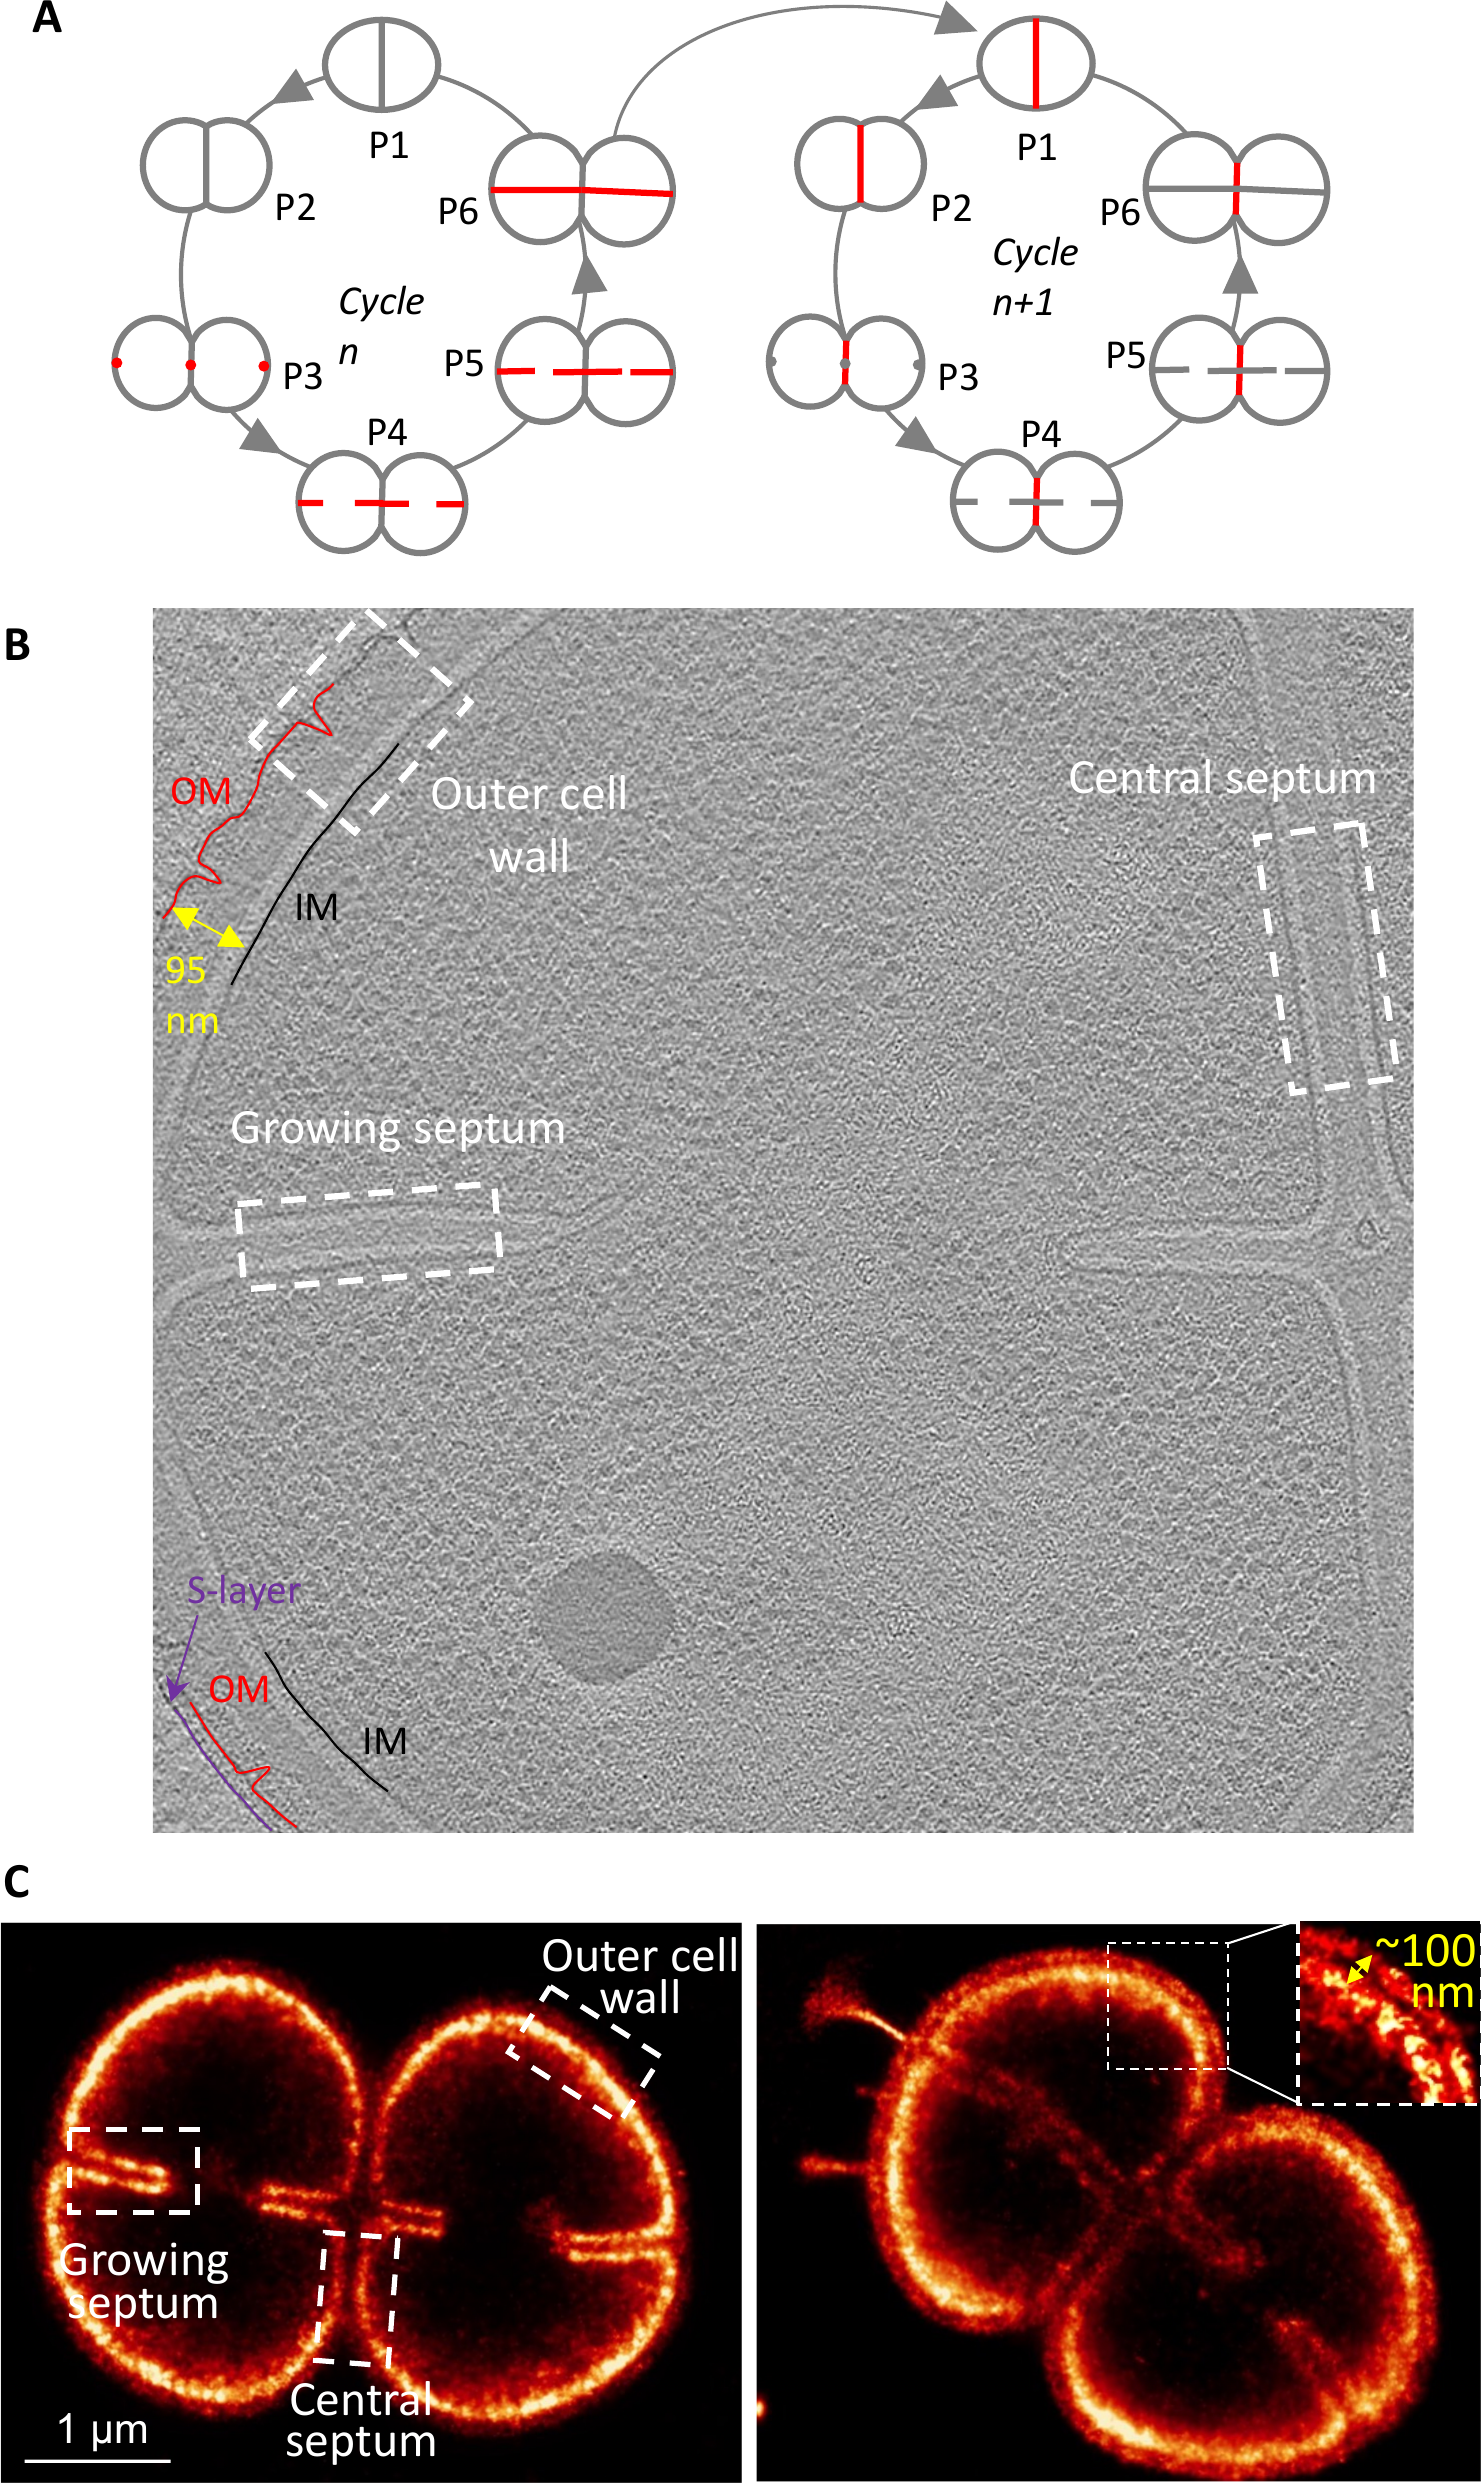
\includegraphics[width=\textwidth]{drad_paper/fig1.png}
    \caption{TODO}
    \label{drad_fig1}
\end{figure}

The outer cell wall bears two lipid bilayers that can be seen as dark lines in the cryo-ET data and could be distinguished on a few occasions in our super-resolved PAINT images of Nile Red stained \textit{D. radiodurans} (\autoref{drad_fig1}B, right panel).
With both techniques, the distance between the inner (IM) and outer (OM) cell membranes was in good agreement and was found to be around \qty{95}{nm} (\autoref{drad_fig1}).
A more in-depth analysis of the cell wall layer composition was facilitated by the preparation of straightened cell wall projections of the cryo-ET images using a recently developed tool, blik~\cite{gaifasBlikExtensible3D2024}.
Density profiles of the outer cell wall revealed that this region was composed of 6 distinct layers: (i) an inner plasma membrane, (ii) a low-density periplasmic region, (iii) a high-density PG layer, (iv) an intermediate layer previously described as the SlpA layer~\cite{vonkugelgenMultidomainConnectorLinks2022}, (v) an outer plasma membrane and (vi) a discontinuous hexagonally packed S-layer on the outer surface of the bacteria (\autoref{drad_fig2}A).
A distinctive white line was seen to separate the PG layer from the SlpA layer and V-shaped invaginations of the outer plasma membrane were seen regularly along this outer cell wall.
Measurements made on numerous cryo-ET datasets allowed us to determine the mean thickness of each of these 6 layers.
When present, the S-layer was typically located at \qty{18}{nm} above the outer cell membrane, the SlpA layer was found to be \qty{34.5}{nm} in thickness in good agreement with the estimated dimensions of the SlpA complex that stretches across this layer~\cite{vonkugelgenMultidomainConnectorLinks2022}.
The PG layer was found to be \sim\qty{42.5}{nm} in thickness and located \sim\qty{15.5}{nm} above the inner membrane with a low-density region located in between these two essential layers.
Interestingly, these measurements revealed that the inner membrane bilayer was significantly thicker than the outer plasma membrane (\qty{5.5}{nm} vs \qty{4.0}{nm}) suggesting distinct lipid compositions.

\begin{figure}[ht]
    \centering
    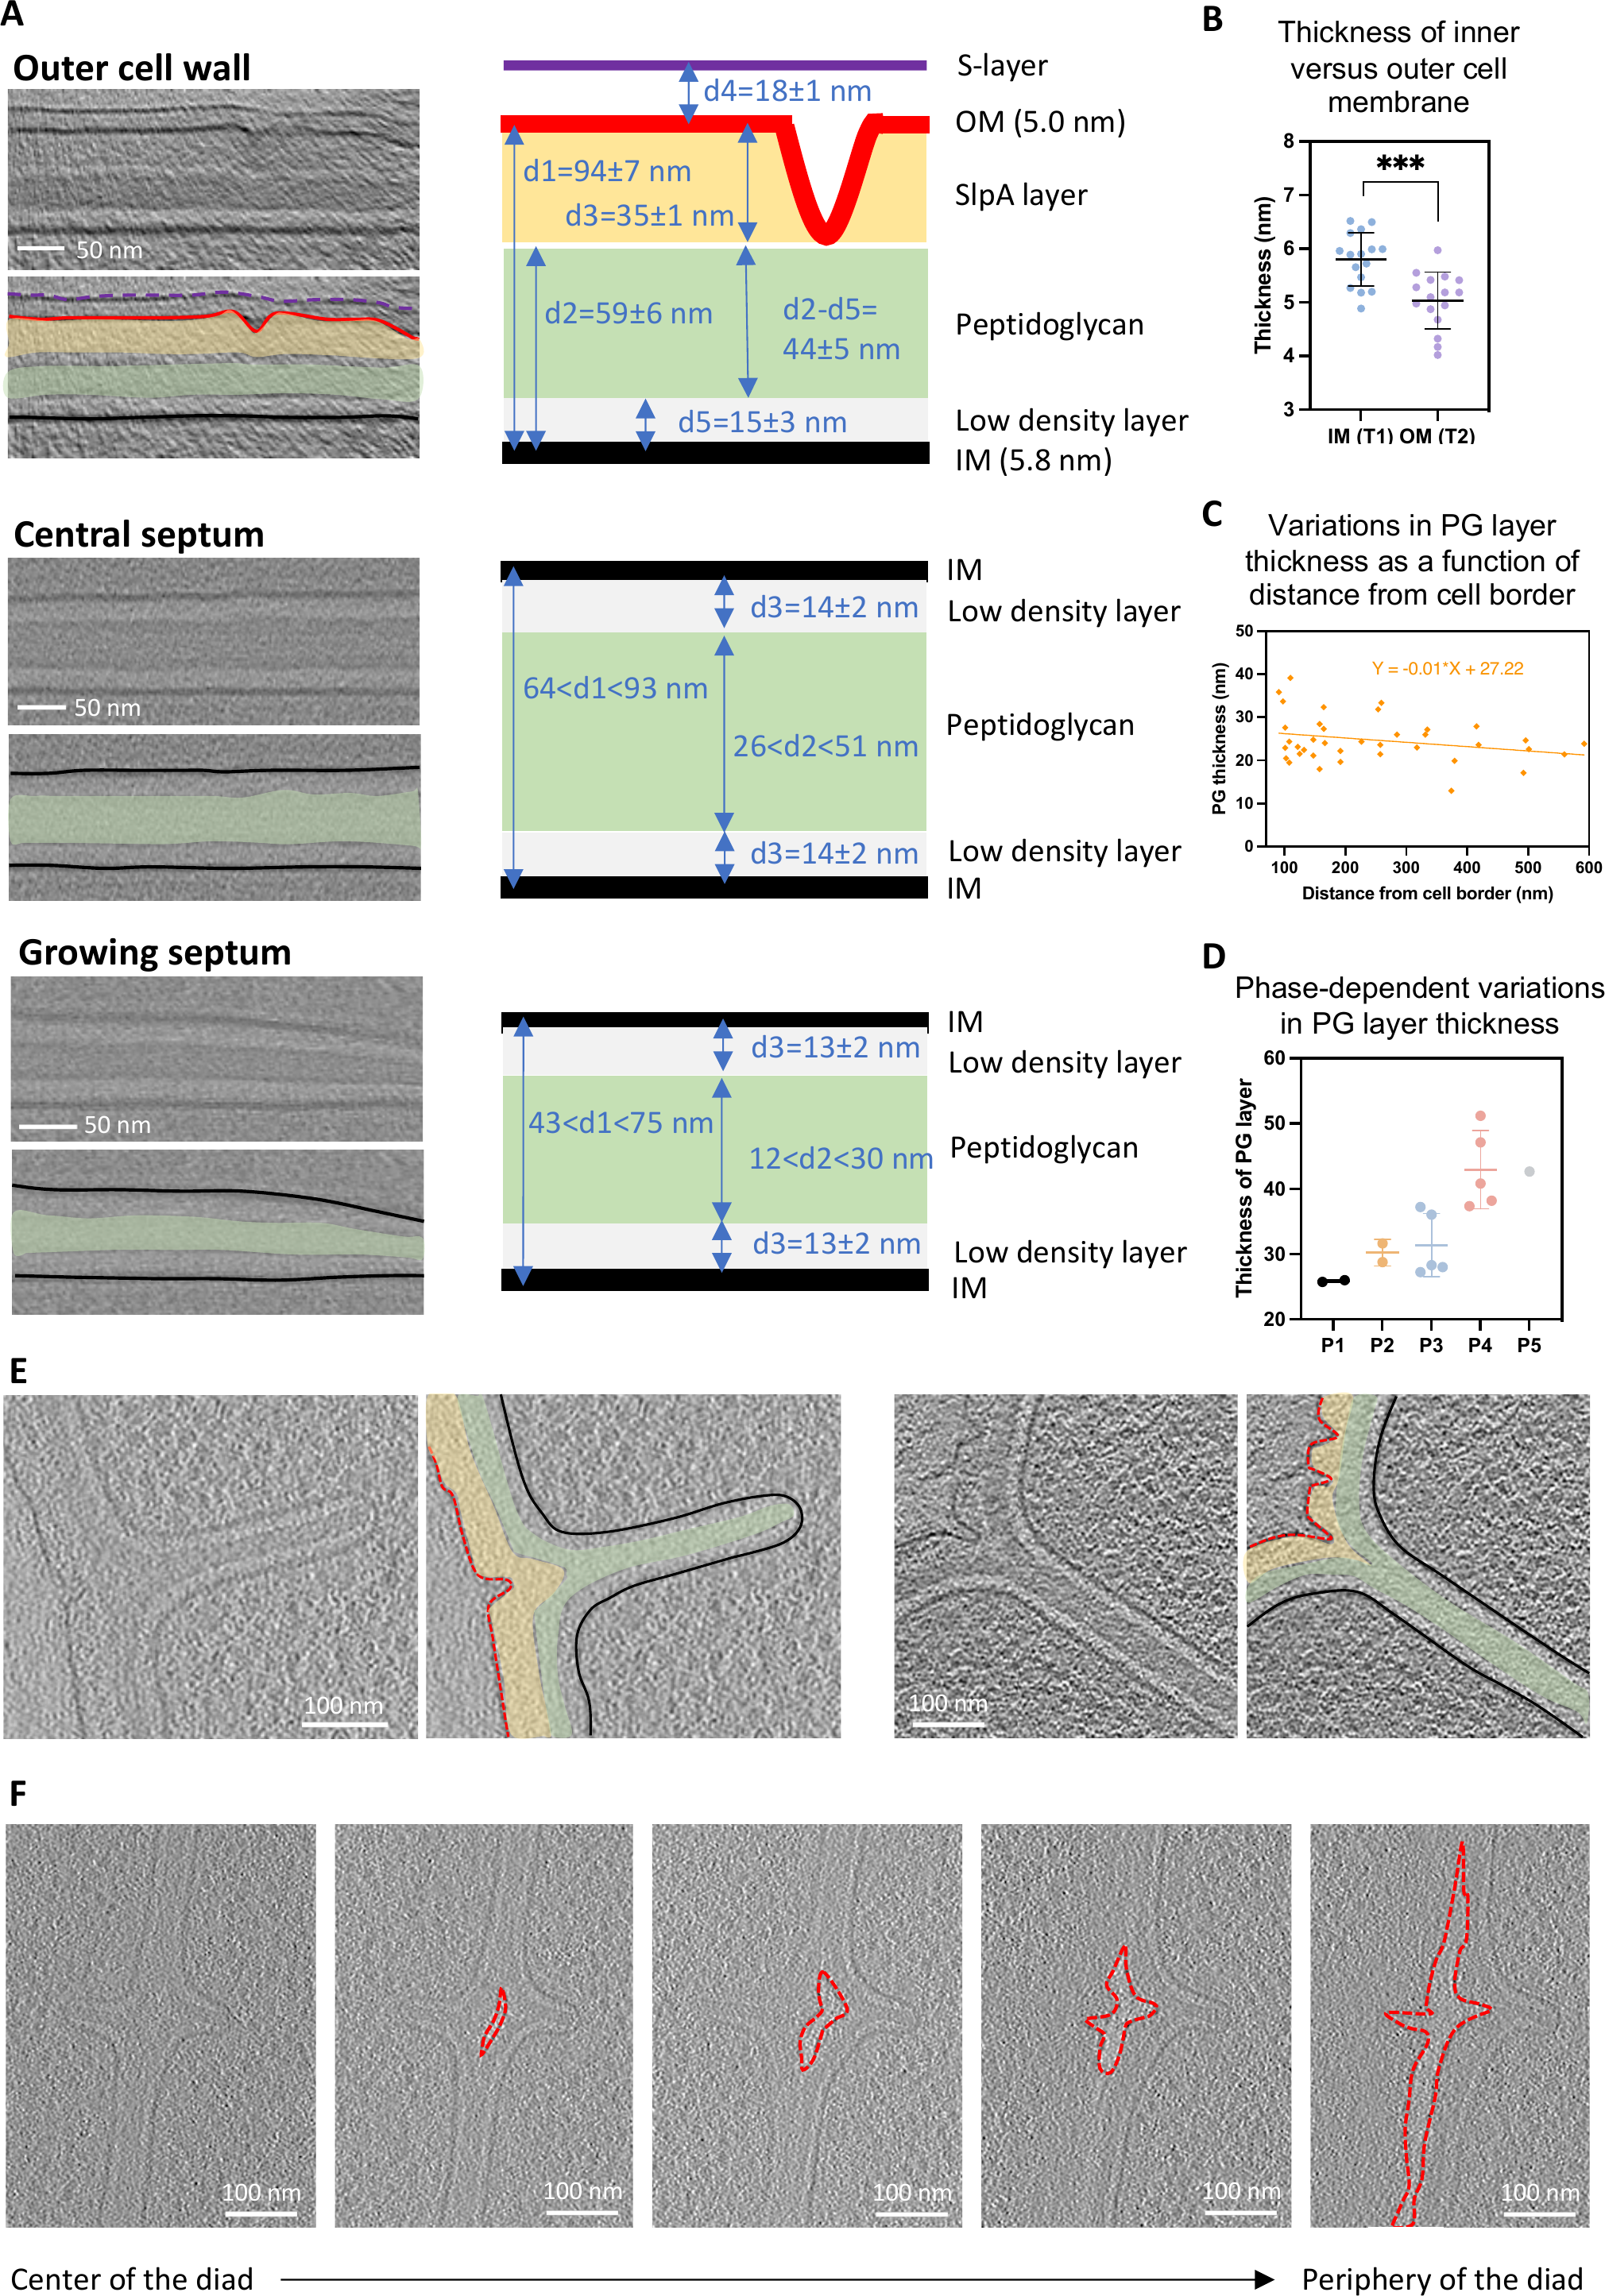
\includegraphics[width=\textwidth]{drad_paper/fig2.png}
    \caption{TODO}
    \label{drad_fig2}
\end{figure}

A similar procedure was used to analyse the composition of the growing septa and the central cell wall region.
The outer layers of the external cell wall were missing in these regions, notably the S-layer, the outer membrane bilayer and the SlpA layer, and instead they were composed of only the inner plasma membrane, the low-density periplasmic region and the PG layer (\autoref{drad_fig2}A).
In contrast to the inner membrane and low-density layers that showed similar thickness in these two locations, the PG layer displayed significant variations, ranging from \qty{42}{nm} to \qty{56}{nm} in the central cell wall and as low as \qty{35}{nm} in the growing septa.
In both the growing septa and the central cell wall, the PG layer was typically thicker at the cell periphery than at the tip of the septum or the centre of the diad respectively, and in the central cell wall, the mean thickness of the PG layer was also found to vary substantially as a function of the phase of the cell cycle, suggesting a progressive thickening of this layer until reaching its definite size prior to the splitting of the diad into two cells (\autoref{drad_fig2}A).

At the junction between the outer cell wall and the growing septum (\autoref{drad_fig2}B and \autoref{drad_sfig2} for more examples), we observed that the PG and low-density periplasmic layers followed the inner membrane, while the outer layers (SlpA layer and outer membrane) were restricted to the outer cell wall.
V-shaped invaginations in the outer membrane were often observed at these junctions and were found to extend inwards during the splitting of the two daughter cells during the subsequent division cycle.
As shown in \autoref{drad_fig2}C, cell splitting is a progressive process, most likely initiated from the cell periphery and moving inwards from both sides of the cell towards the center of the diad forming bubble-like membrane structures (\autoref{drad_sfig1}B for more examples).
Splitting occurs concomitantly with the addition of the SlpA layer and finally the outer cell membrane to the central septum cell wall to protect the cells from the external environment (\autoref{drad_fig2}C).

\FloatBarrier

\subsection{Structure of septal tips}

A close inspection of the tomograms revealed that the tips of the growing septa exhibited particular structures.
A majority of septa (40 of the 64 septa visible in our tomograms) were slightly tapered at their tips and the low-density periplasmic region was significantly thinner in these regions bringing the PG layer very close to (in some cases even touching) the inner membrane (\autoref{drad_fig3}A).
Strikingly, in nearly 40\% of the observed septa, membrane protrusions, reported in earlier studies as mesosomes~\cite{thornleyFineStructureMicrococcus1965,sleytrStudyFreezeetchingFine1973}, were observed at the tips of growing septa (\autoref{drad_fig3}B-C and \autoref{drad_sfig2} for more examples).
These structures are composed solely of the low-density layer and are delimited by the inner membrane.
They were in a large majority of cases observed in cells in early stages of the septation process bearing short septa.
These extensions were found to adopt either extended tube-like structures or more circular loop-like structures.
In all cases, they appeared to be very flexible, probably as a result of the absence of a PG layer to rigidify the extension.
This intrinsic flexibility may explain why the tips of the growing septa were often not observed in the super-resolved images of Nile Red-labelled \textit{D. radiodurans} cells (\autoref{drad_fig3}C, left panel).
Instead, in these images, open ends were observed at the septal tips, suggesting that either the Nile Red dye poorly labelled these highly curved membrane bilayers or that the tips were very mobile and not captured in live imaging experiments.
Both of these phenomena may also be at play.
On a few occasions, we did observe more poorly defined Nile Red labelling at the tips of growing septa that may correspond to these flexible membrane protrusions (\autoref{drad_fig3}C, right panel).

\begin{figure}[ht]
    \centering
    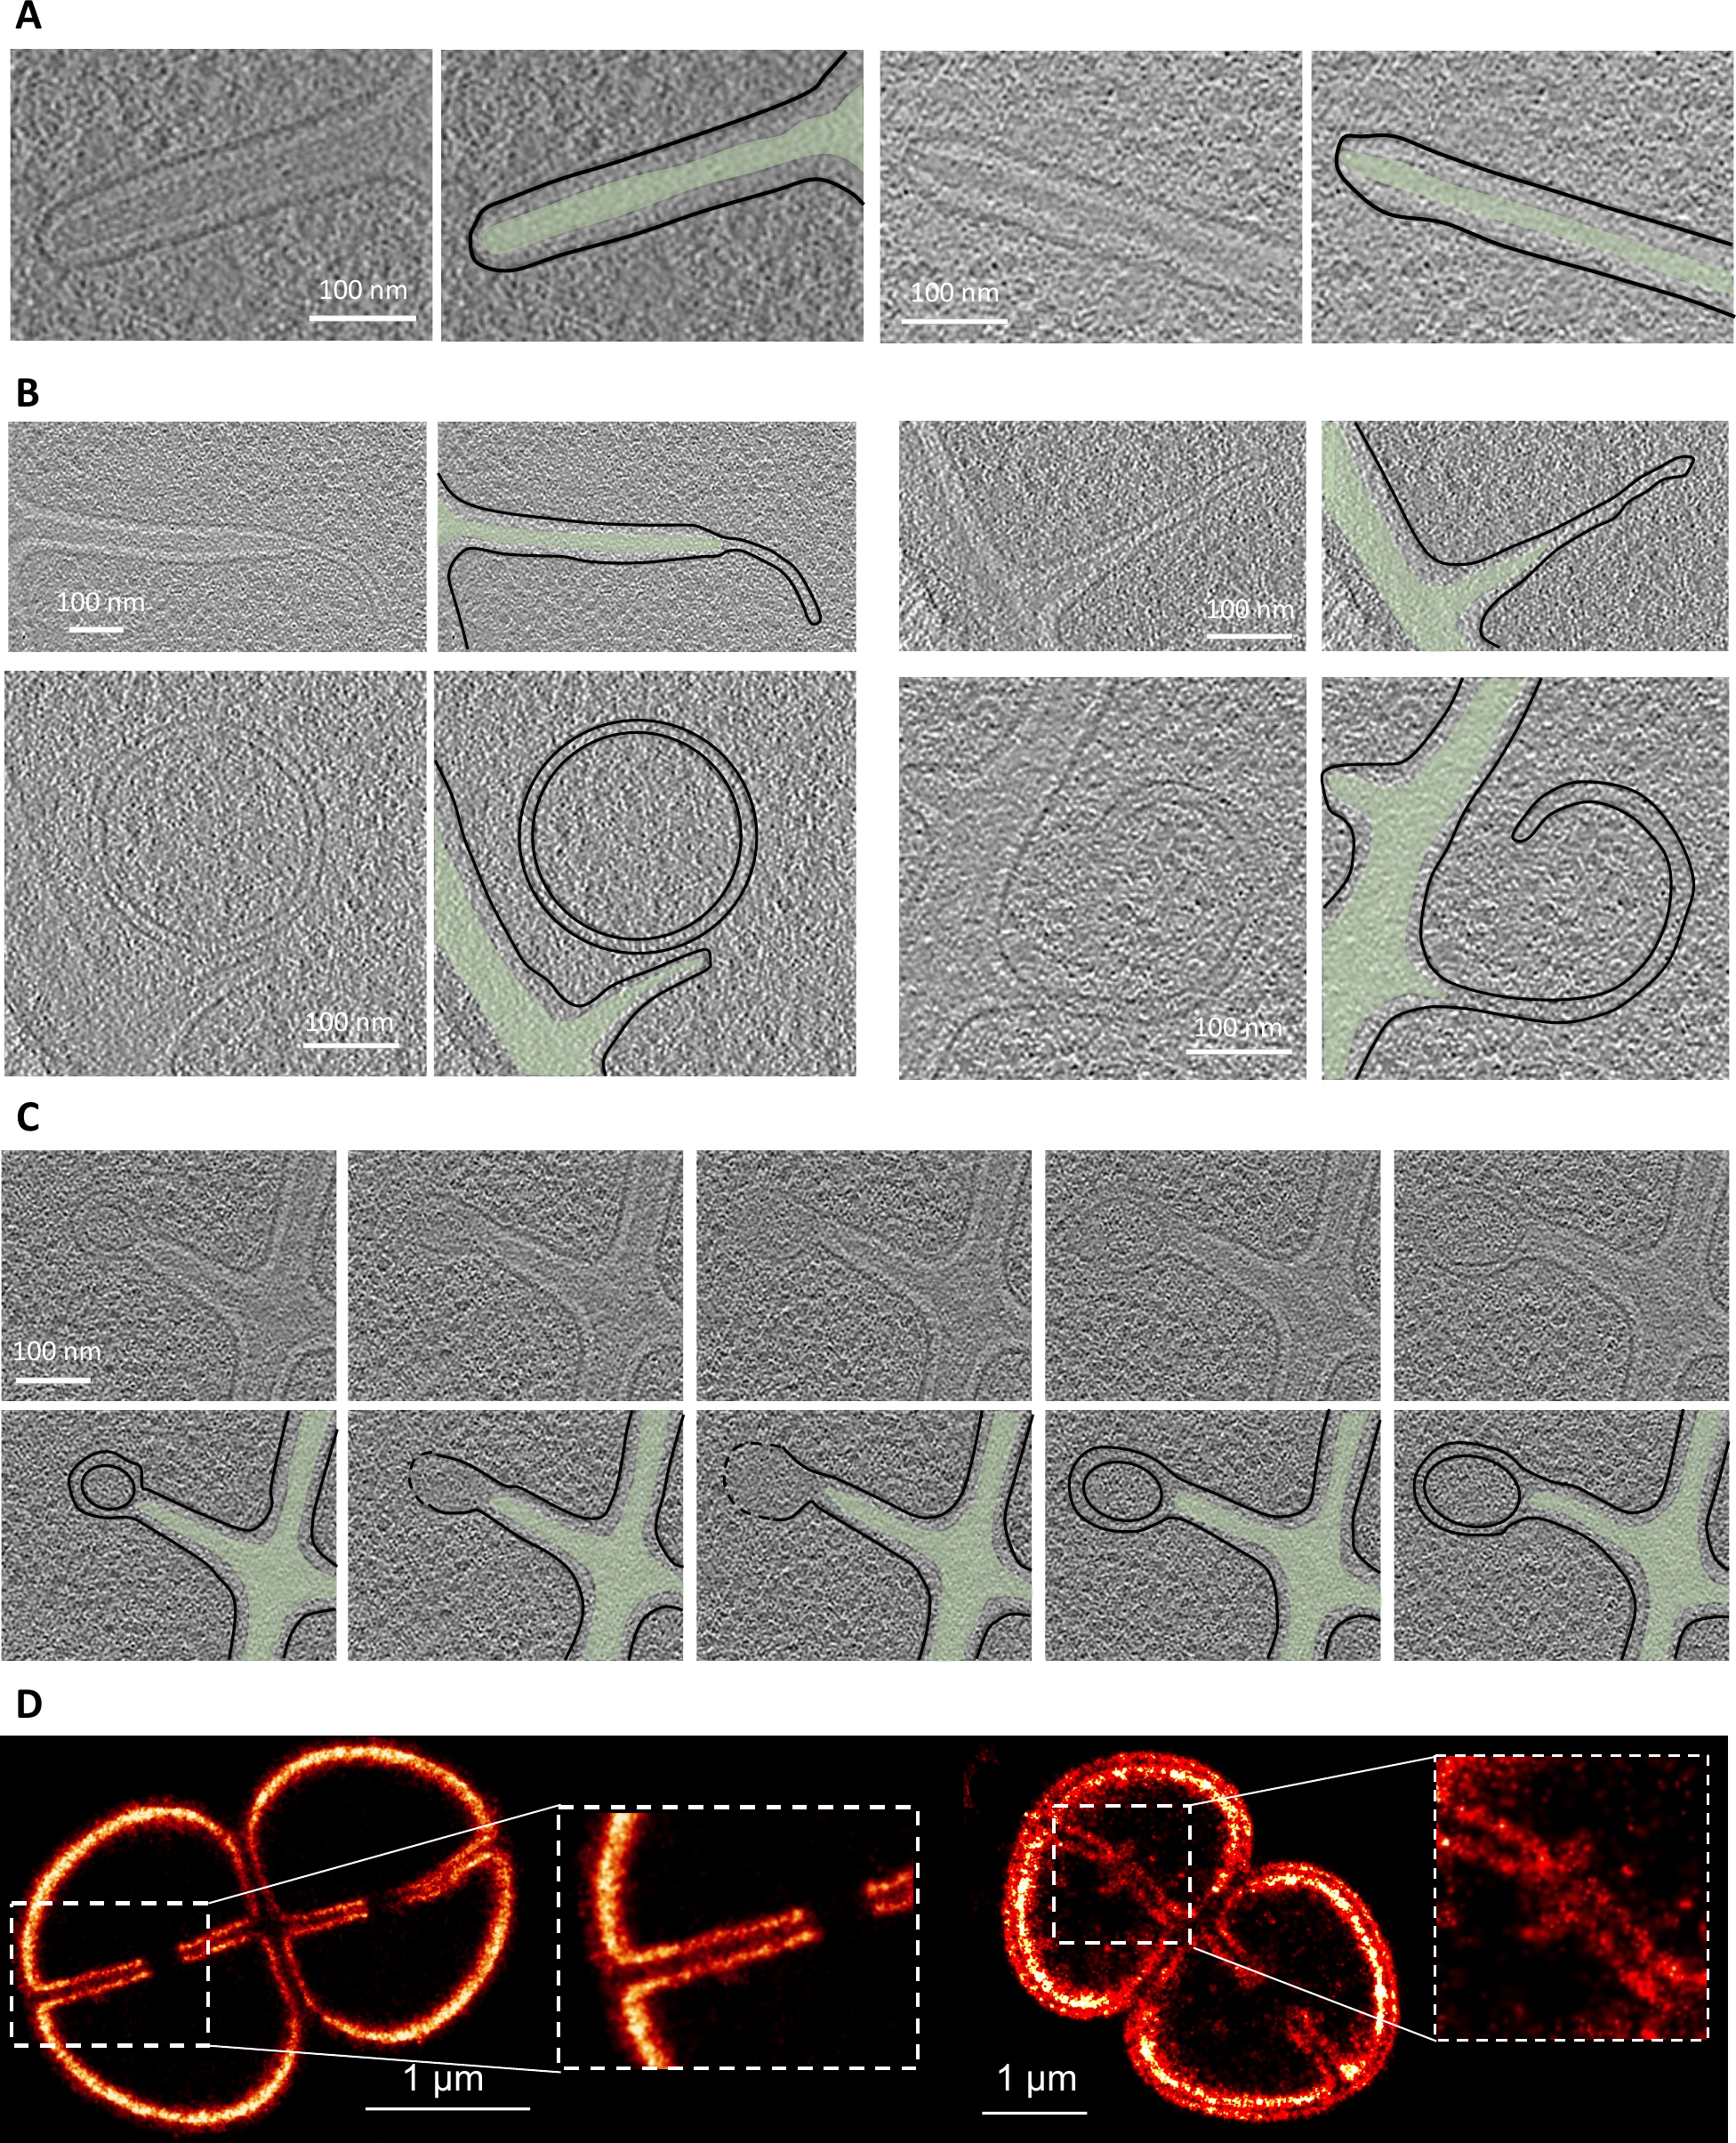
\includegraphics[width=\textwidth]{drad_paper/fig3.png}
    \caption{TODO}
    \label{drad_fig3}
\end{figure}

\FloatBarrier

\subsection{Septation through a "sliding door" mechanism}

Using timelapse 3D video confocal microscopy of Nile Red stained \textit{D. radiodurans} bacteria immobilized in various orientations on agarose pads (\autoref{drad_sfig3}), we followed the division process in live cells (SI videos 1 and 2).
Septation was found to involve several steps.
First, two septa originating from opposite sides of the cell grow inwards with a flat leading edge creating a central gap stretching from the top to the bottom of the cell.
As the septa grow, the leading edge progressively becomes more curved forming a cat's eye structure in between the two opposite septa.
Finally, when the two septa come close to each other, fusion starts first at the top and bottom of the cell and then rapidly proceeds through a zipping mechanism from the cell periphery to the cell center.
3D PAINT images of Nile Red labelled \textit{D. radiodurans} cells confirmed these observations, allowing to capture high-resolution images of dividing cells exhibiting septa with flat or slightly curved leading edges embracing a central gap that stretches all across the cell (\autoref{drad_fig4}A).
Kymographs of individual septation events were extracted from the live cell confocal acquisitions to probe the kinetics of this process (\autoref{drad_fig4}B).
These revealed that septation is a linear process in which the external and internal septa grow respectively at rates of \qty{7.3(0.5)}{nm.min^{-1}}  and \qty{4.1(0.7)}{nm.min^{-1}} until full closure.
Interestingly, the external septum starts growing ahead of the internal septum, as can be seen from the asymmetric V-shaped structure of the kymographs, and grows at a faster rate than the internal septum (\autoref{drad_fig4}B).
This may be explained by the fact that the external septum needs to grow further than the internal septum to reach the site of fusion located at mid-cell and has to compensate for the expansion of the cells that is occurring simultaneously (\autoref{drad_fig4}A).
A flat leading edge and an asymmetric growth of the external and internal septa were also observed in our cryo-ET data, which captured bacteria at various stages of the division process (\autoref{drad_fig4}C-D).

\begin{figure}[ht]
    \centering
    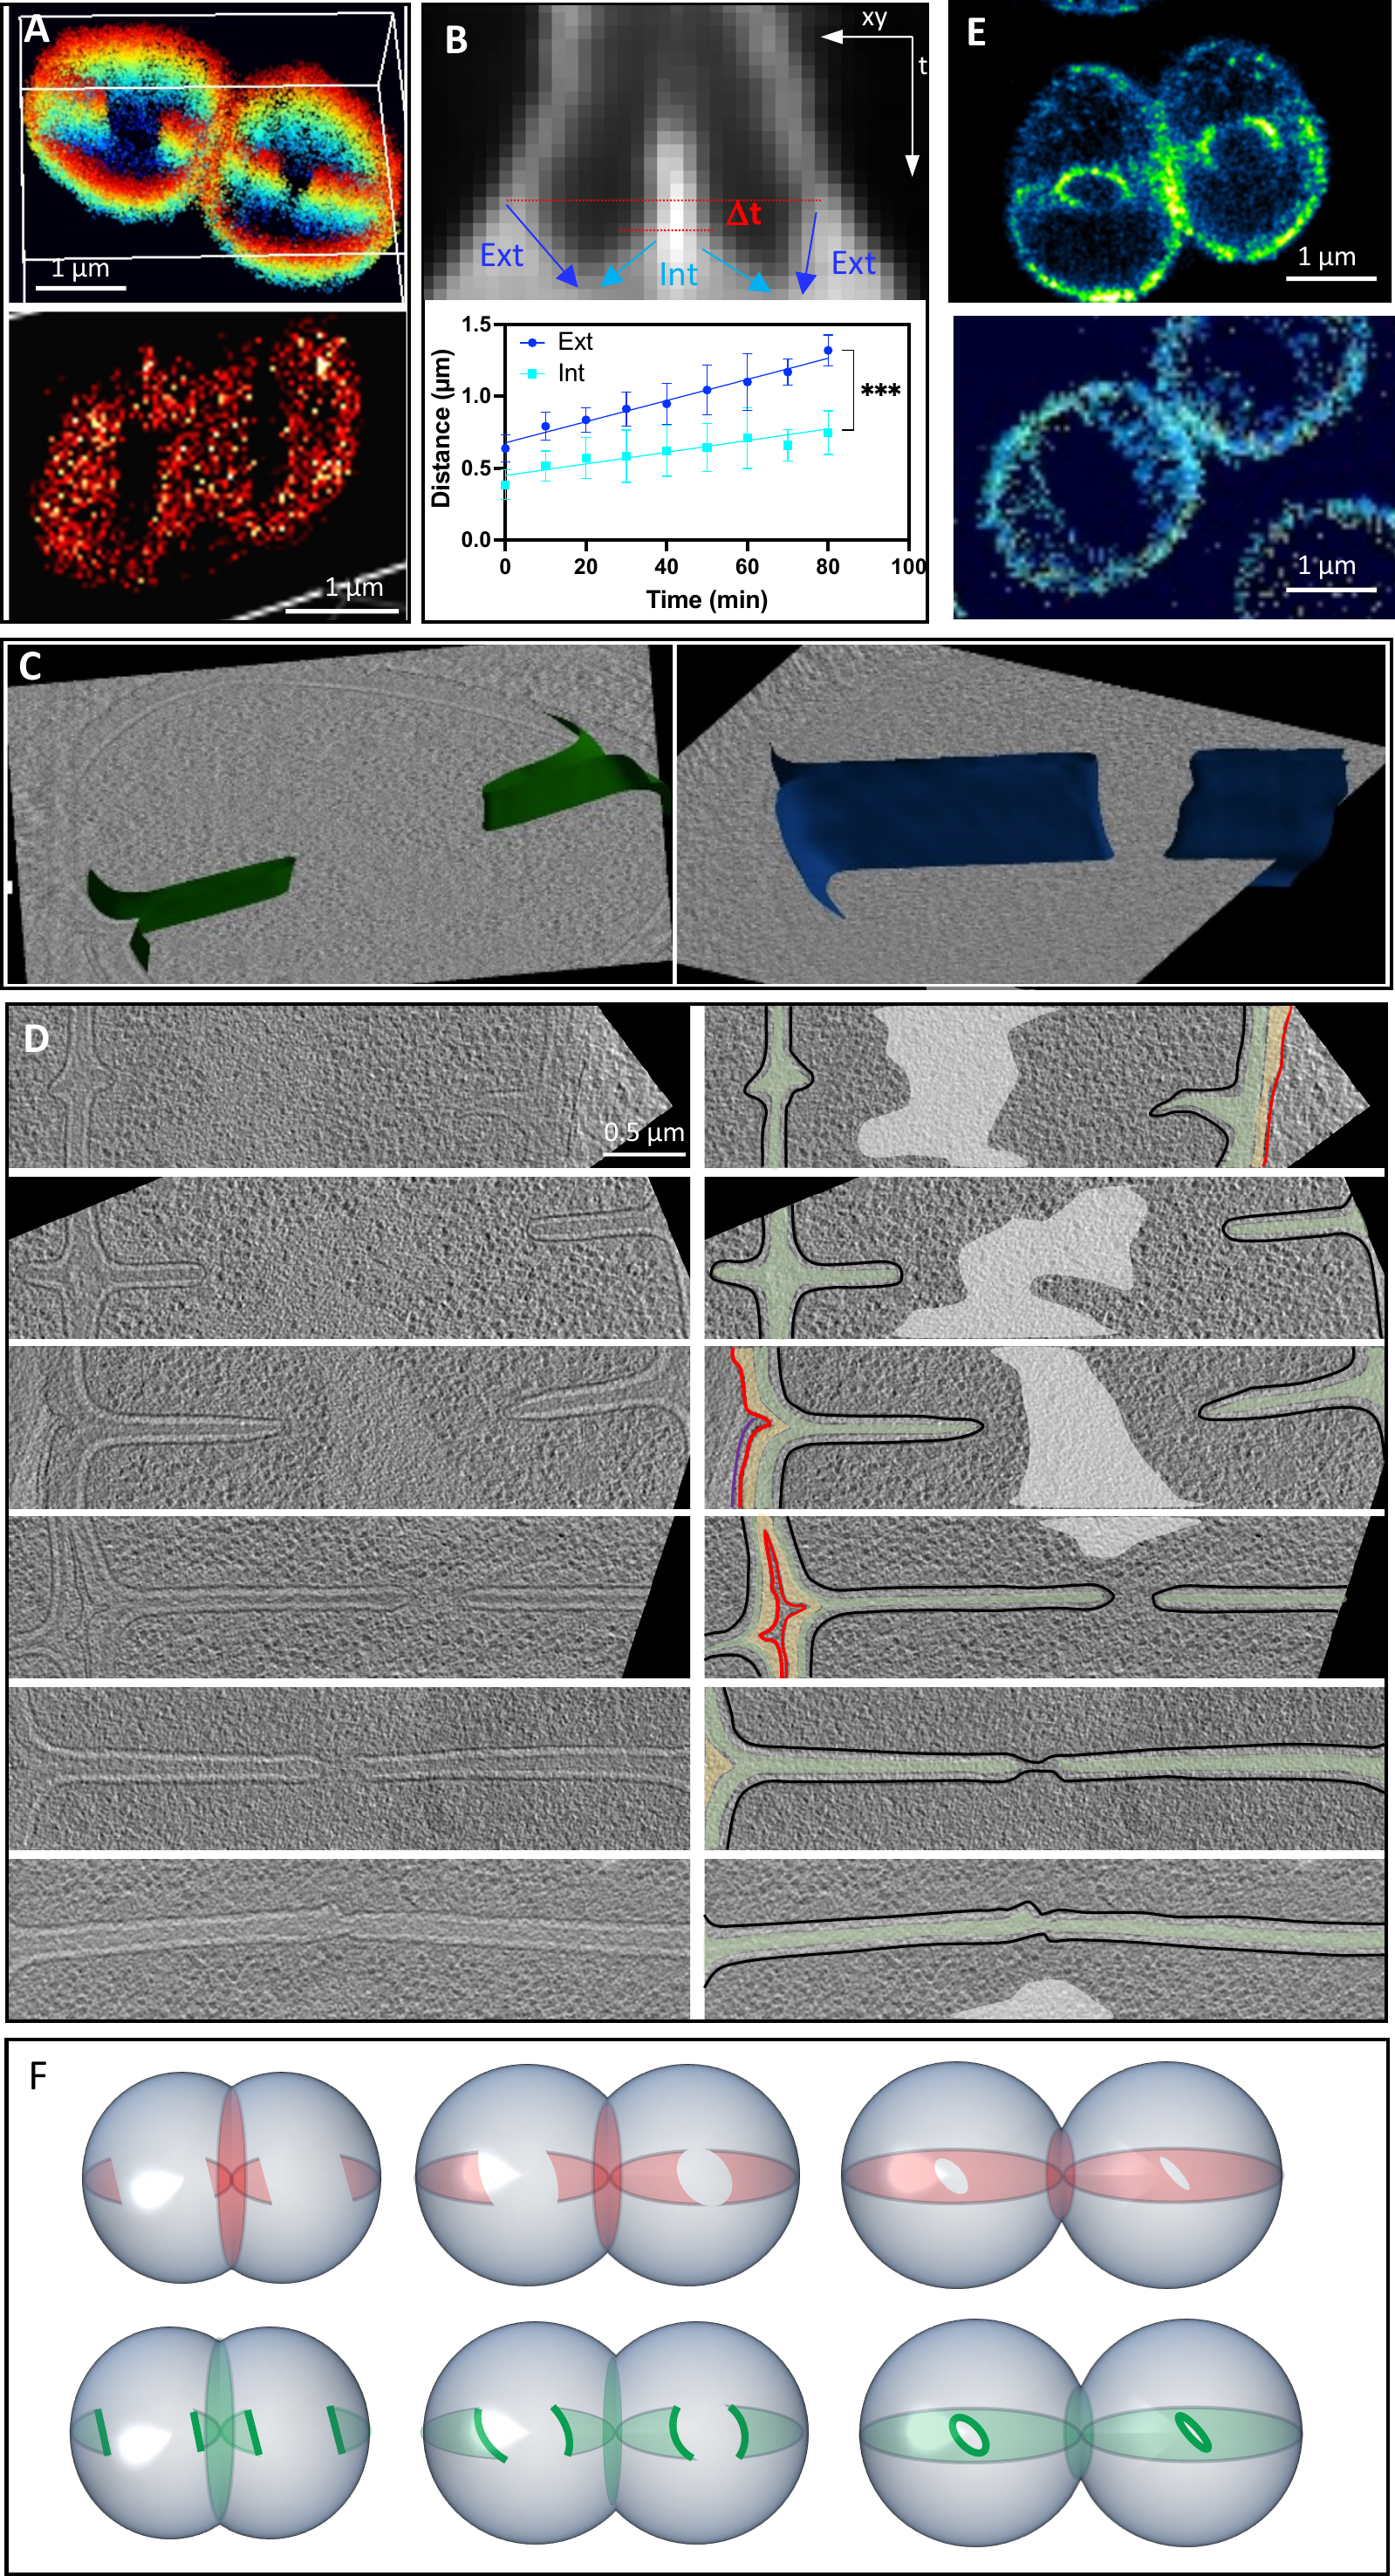
\includegraphics[width=.8\textwidth]{drad_paper/fig4.png}
    \caption{TODO}
    \label{drad_fig4}
\end{figure}

In addition to staining the cell membrane, we also labelled the PG layer of \textit{D. radiodurans} cell walls by incorporating modified D-alanine (zDA) into the cell wall that was subsequently labelled by click chemistry with fluorescent probes suitable for either confocal or dSTORM microscopy (\autoref{drad_sfig4}).
The PG labelling pattern (\autoref{drad_fig4}E and \autoref{drad_sfig5}) was very similar to that of Nile Red labelled cells, with an efficient incorporation occurring in all regions of the cell wall (septal, central and outer cell walls).
The main difference was that the PG labelling was more prominent at the leading edge of the growing septa than elsewhere, suggesting this likely corresponds to the major site of active PG synthesis in these dividing cells (\autoref{drad_fig4}F).
This is particularly visible at late stages of the cell cycle, either just before (Phase 5) or just after cytokinesis (Phase 6), where an intense band of labelled PG can be seen at the site of fusion where the two opposing septa meet (\autoref{drad_sfig5}C).
In agreement with these observations, pulse-chase experiments in which bacteria were returned to the incubator for 45 minutes (chase) after incorporation of the modified D-Alanine (pulse) into their cell walls, revealed that septa having incorporated zDA labelling at their tips during the pulse period, were progressively extended further by unlabelled PG, indicating that new PG is added to the existing layer in an inwards direction until the opposing septa are close enough to fuse (\autoref{drad_fig4}F and \autoref{drad_sfig6}).

Close examination of the tomograms also revealed that the position and shape of the growing septa changed as a function of their length (\autoref{drad_fig4}D).
At early stages of the septation process, short septa were not always precisely facing each other and their tips were often bent and bearing membrane extensions, while at later stages, septa were remarkably straight and fully aligned to ensure fusion of the septa originating from opposite sides of the cell.
The presence of a PG layer in the growing septa appears to be a pre-requisite for the formation of these straight and well-aligned septa, indicating that the synthesis of the PG layer may provide the necessary rigidity to the growing cell walls for the final closure.
This final fusion step was captured in two of the tomograms and was found to proceed first through fusion of the lipid bilayers (highlighted in red in \autoref{drad_fig4}D) and subsequently through synthesis of PG to fill the gap and "glue" the two septa together.
Taken together, these data allow us to propose a model for septation through the "sliding doors" mechanism, which is illustrated schematically in \autoref{drad_fig4}F.

\FloatBarrier

\subsection{PG synthesis in the outer cell wall and in the septa are performed by distinct machineries}

To better understand the molecular mechanisms underlying this unusual mode of septation, we treated \textit{D. radiodurans} cultures with the \beta-lactam antibiotic, ampicillin, and compared the growth of untreated and treated Nile Red labelled cells by 3D confocal timelapse microscopy for a three-hour period (SI videos 3 and 4).
Ampicillin is known to bind to the active sites of certain PBPs, thereby inhibiting their enzymatic cell wall synthesis function~\cite{sauvageGlycosyltransferasesTranspeptidasesPenicillinBinding2016}.
To our surprise, septation but not cell growth was arrested by ampicillin treatment (\autoref{drad_fig5}).
Indeed, the growth of the outer cell perimeter was unaffected by this treatment during this three-hour period, while growth of both the internal and external septa were rapidly arrested (\autoref{drad_fig5}B-C).
After 1 hour, the septa even started to shorten, suggesting they may be undergoing disassembly and degradation (\autoref{drad_fig5}C).
As a result of this change in the balance between cell growth and septation, cells progressively became distorted (more elongated with a slight bulge at sites of division) as evidenced by the substantially increased diameter (d) to perimeter (p) ratio after three hours of treatment with ampicillin (\autoref{drad_fig5}D).
The specific inhibition of septal growth by ampicillin suggests that the PBPs responsible for PG synthesis and maturation in the septa are distinct from those involved in outer cell wall growth.

\begin{figure}[ht]
    \centering
    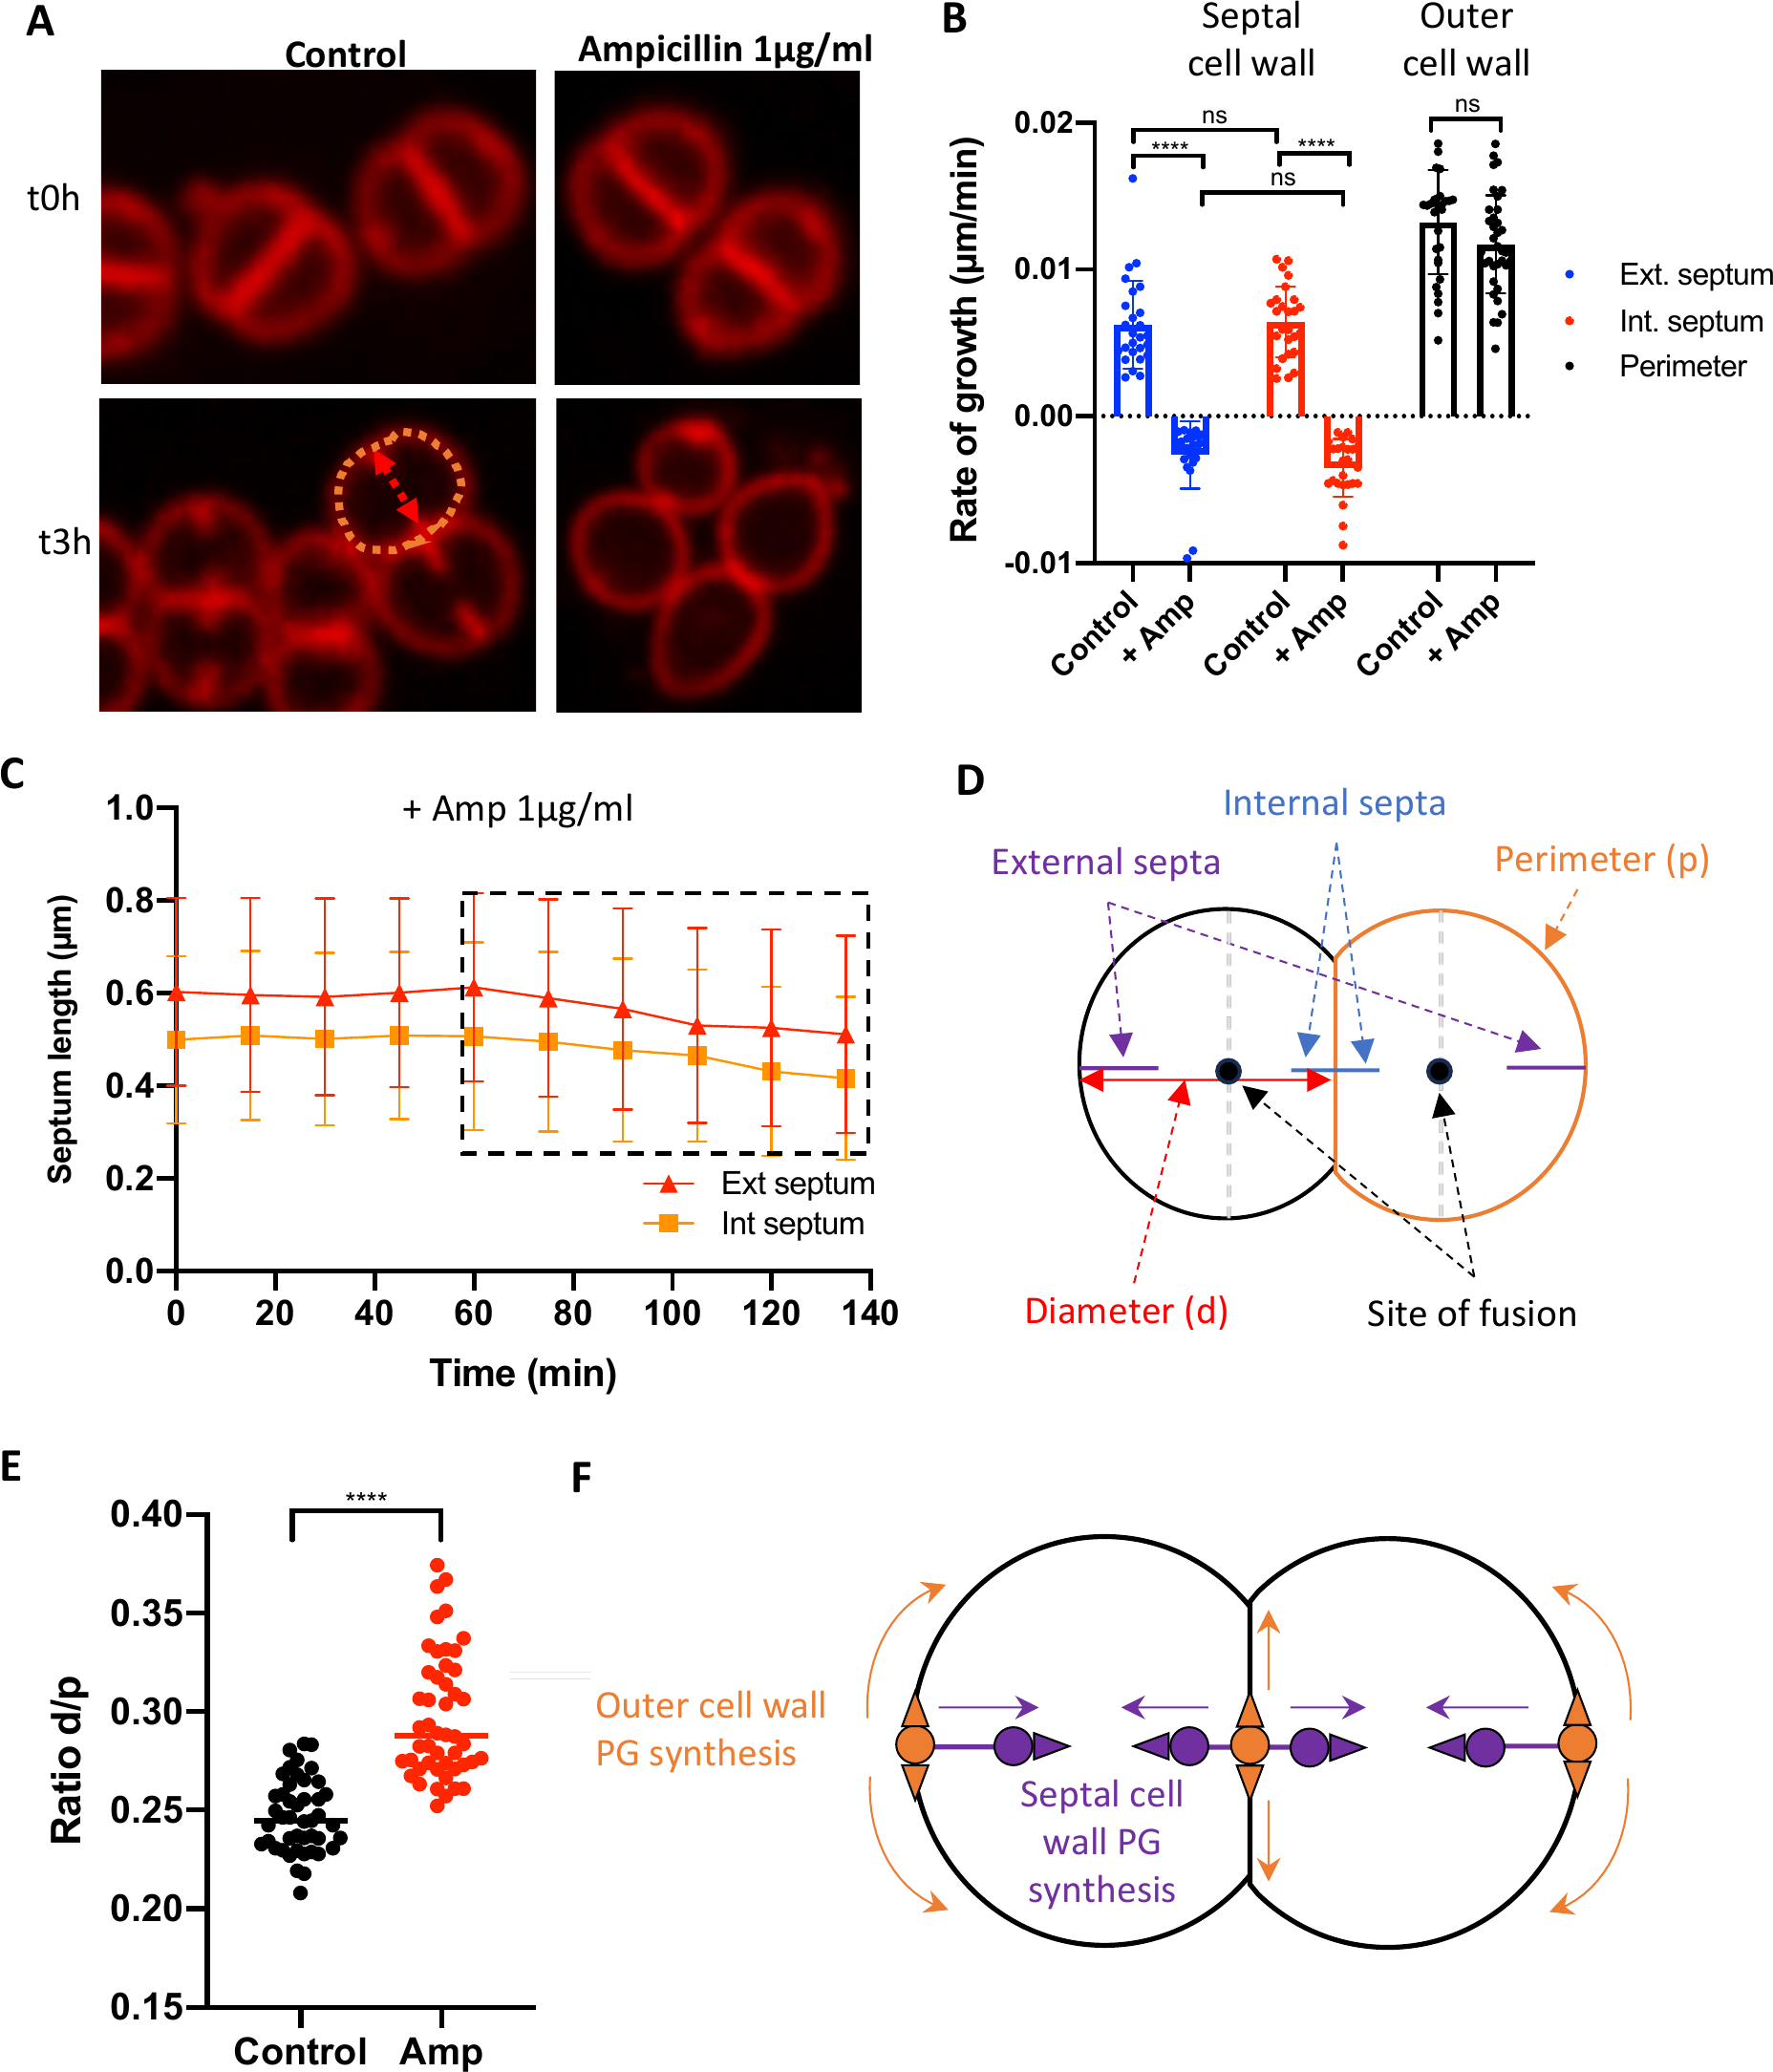
\includegraphics[width=.8\textwidth]{drad_paper/fig5.png}
    \caption{TODO}
    \label{drad_fig5}
\end{figure}

Next, we repeated the zDA incorporation experiment on cells pre-grown for either 1 or 2h in the presence of ampicillin before the labelling (\autoref{drad_sfig7}).
In these conditions, zDA was still readily incorporated into the outer cell wall, as expected based on our timelapse experiments.
In contrast, no labelling was seen in the septal regions except at sites of septation initiation, where a distinctive bright PG-labelled ring was observed (\autoref{drad_sfig7}).
These rings were occasionally seen in untreated cells (\autoref{drad_sfig_missing}), but were much more abundant in ampicillin-treated cells and in particular in samples pre-grown for 2 hours in the presence of the \beta-lactam antibiotic, where approximately 50\% of the cells displayed such ring-shaped PG labelling (\autoref{drad_sfig7}B).
The initial PG synthesis at the start of septation thus appears to be unaffected by ampicillin, while subsequent growth and extension of the septa is fully arrested by this treatment.
A shared PG machinery located at the junction between the outer cell wall and the start of septation may therefore be involved in both outer cell wall synthesis and initiation of septation, but a distinct set of proteins likely located at the tip of the growing septa appear to be responsible for PG synthesis across the dividing cells (\autoref{drad_fig5}E).
This finding is supported also by the pulse-chase experiments (\autoref{drad_sfig6}) in which we observed that most of the labelling of the septal regions, but not of the outer cell walls was lost after the chase period, indicating that the PG structure and/or maturation process are quite distinct in these two types of cell wall.

\FloatBarrier

\subsection{FtsZ is present at the tips of septa}\label{drad_ftsz}

We investigated the location of FtsZ, one of the key players in bacterial cell division, in dividing \textit{D. radiodurans} cells using both fluorescence microscopy and cryo-ET.
Two strategies were used to label FtsZ: (i) immunolabelling of an endogenously HA-tagged FtsZ or (ii) endogenous tagging of FtsZ with a photoconvertible fluorescent protein, mEos4B.
The latter was compatible with live cell imaging, but this genetically modified strain of \textit{D. radiodurans} showed altered cell morphology (forming many large cells with likely impaired septation) and only a small fraction of cells exhibited fluorescence signal and visible Z-rings (\autoref{drad_fig6}A).
In contrast, the strain expressing HA-tagged FtsZ grew very well with no obvious morphological defects and FtsZ could be detected after fixing and permeabilizing the cells with an anti-HA antibody by either confocal or dSTORM microscopy (\autoref{drad_fig6}A-B).
Both strategies indicated that \textit{D. radiodurans} FtsZ forms ring- or oval-shaped structures of various sizes as reported for other bacteria, some of which appear to be incomplete.
Dual labelling of FtsZ and the cell membrane also revealed that FtsZ locates to the tip of growing septa at all stages of septation, including very early stages when septa are not yet visible by fluorescence microscopy (\autoref{drad_fig6}B).
At these early stages, FtsZ appeared to form arches rather than complete rings.

\begin{figure}[ht]
    \centering
    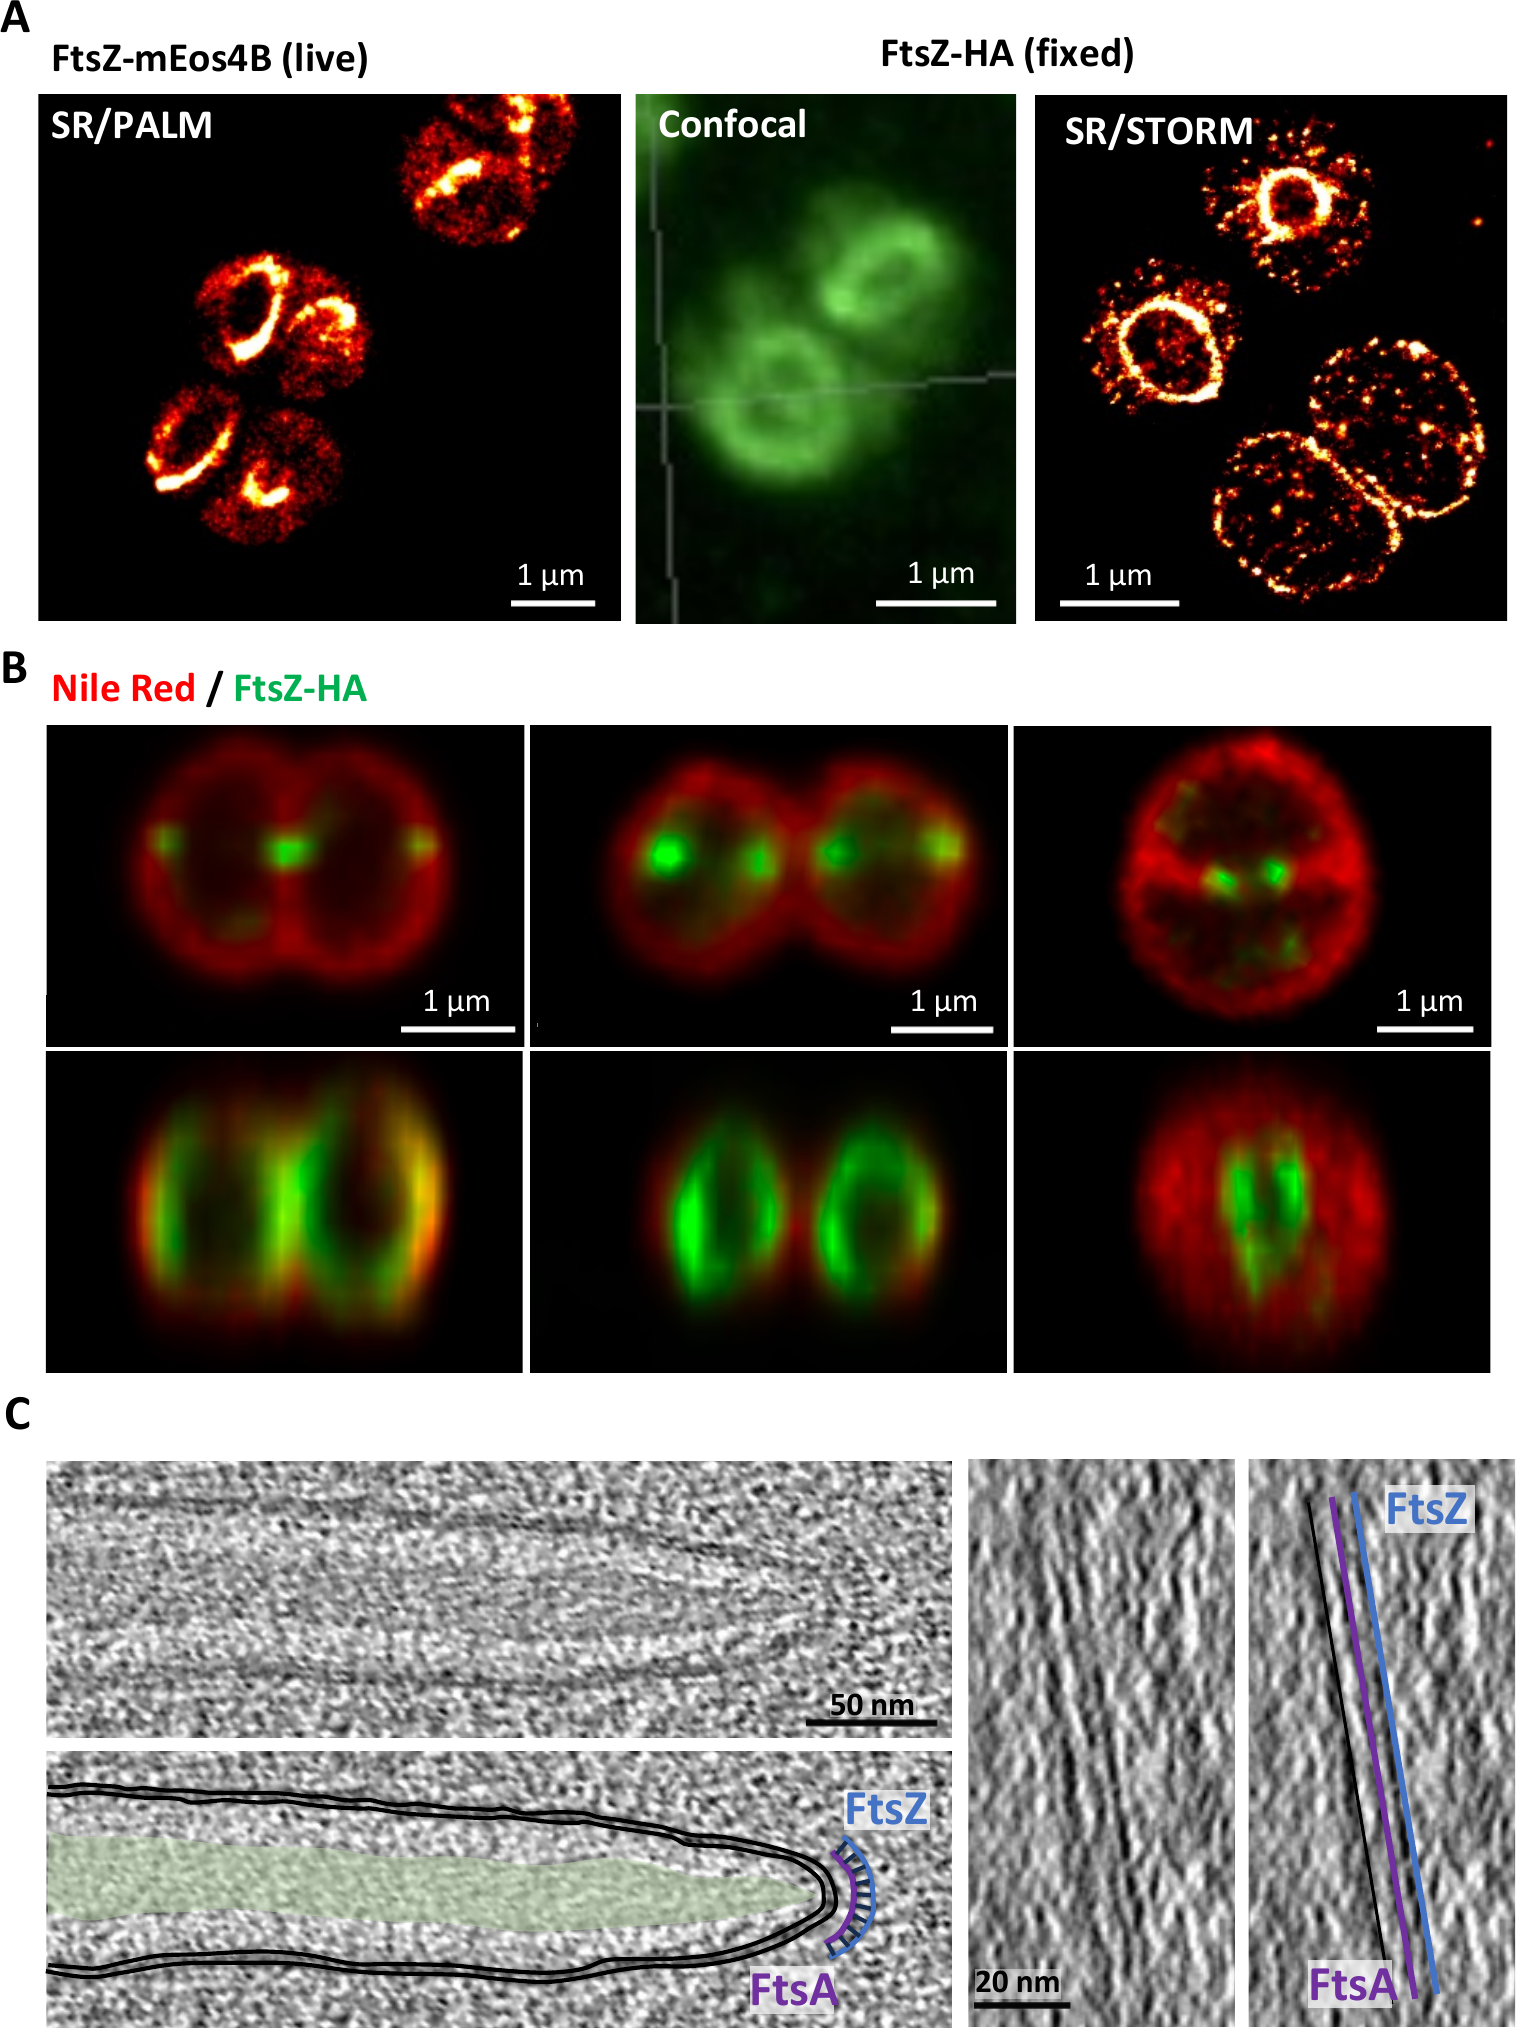
\includegraphics[width=\textwidth]{drad_paper/fig6.png}
    \caption{TODO}
    \label{drad_fig6}
\end{figure}

Examination of the tomograms revealed the presence of a double-arched structure situated at \sim\qty{15}{nm} from the septal tip, which likely corresponds to FtsZ (outer arch) and its cellular partner the membrane-bound FtsA~\cite{sextonSuperresolutionConfocalCryoCLEM2022} (inner arch; \autoref{drad_fig6}C).
These structures were again observed at all stages of the septation process as in our fluorescence microscopy data, and when looking at the z-projection, they were found to form long straight filaments characteristic of FtsZ.
Interestingly, FtsZ was not detected when septa were extended with membrane structures, suggesting that FtsZ only assembles at septal tips containing PG in close proximity to the membrane.
However, FtsZ was sometimes seen either above or below these membrane extensions, forming a discontinuous filament, which may explain the incomplete ring structures observed by fluorescence microscopy (\autoref{drad_fig6}A-B).

\FloatBarrier

\section{Discussion}

TODO: Brief summary of results.

\textit{D. radiodurans} is a spherical diderm bacterium that is known to possess a unique cell envelope including an outer S-layer, which has been the object of numerous studies over the past decades~\cite{vonkugelgenMultidomainConnectorLinks2022,workMorphologyChemistryCell1968,rothfussInvolvementSlayerProteins2006,vonkugelgenInterdigitatedImmunoglobulinArrays2023,farciSDBCActiveQuenching2023,farciStructuredOrganizationDeinococcus2022,farciCryoEMStructureSlayer2022,farciStructuralAnalysisArchitecture2021,baumeisterThreedimensionalStructureRegular1986,baumeisterStructureCellEnvelope1981}.
Bacteria from the \textit{Deinococcus-Thermus} phylum, such as \textit{D. radiodurans}, exhibit features of both Gram positive and Gram negative bacteria.
\textit{D. radiodurans} is indeed lacking lipopolysaccharides typically found in Gram negative bacteria, possesses a thick PG layer (\qty{35}{nm}-\qty{55}{nm}) characteristic of Gram positive bacteria and yet its cell envelope is composed of two membrane bilayers characteristic of Gram negative bacteria~\cite{guptaOriginDidermGramnegative2011}.
The exact composition and structure of this unusual cell wall has been the object of much controversy in the recent years, notably regarding the outer layers linking the PG to the outermost S-layer hexameric lattice structure.
Our cryoET analysis of the outer cell wall composition fully supports the model proposed by Bharat and colleagues, in which the whole cell wall is \sim\qty{100}{nm} in thickness and composed of two membranes in between which can be found a thin periplasmic space and two thicker layers, the PG and SlpA layers~\cite{vonkugelgenMultidomainConnectorLinks2022}.
The S-layer is then located \sim\qty{18}{nm} above the outer membrane~\cite{vonkugelgenInterdigitatedImmunoglobulinArrays2023}.
The SlpA layer takes its name from the major protein constituent of this layer, the SlpA protein, a trimeric porin-like protein that is embedded in the outer membrane and stretches across the SlpA layer via a long coiled-coil region to connect to the PG layer~\cite{vonkugelgenMultidomainConnectorLinks2022}.
The predicted length of this assembly (\sim\qty{28}{nm}-\qty{29}{nm}) is in good agreement with our estimated thickness of the SlpA layer (\qty{35}{nm}).
Interestingly, we observe a distinctive white line between the PG and SlpA layers that may correspond to the sites at which the N-terminal SLH domain of SlpA attaches to the PG layer.

\subsection{Cell wall structure and composition} -- discuss earlier studies by Piano et al and Bharat et al.

\subsection{Progressive splitting of cells by action of hydrolases} -- tight coupling with synthesis of outer layers.

\subsection{Septation process} -- Closing door mechanism \& progressive filling of membranes to form rigid septa.
Distinct PG synthesis machinery in septa and in outer cell wall.
Outer cell wall machinery may be largely located at junction of septum and outer cell wall whereas septum-specific machinery is located at tip of growing septa.

Mesosomes: Similar structures were reported in early studies of \textit{D. radiodurans}~\cite{thornleyFineStructureMicrococcus1965,sleytrStudyFreezeetchingFine1973} and other model bacteria~\cite{suganumaStudiesFineStructure1966,pontefractMesosomesEscherichiaColi1969} in the 1960's, but were later considered as artefacts of chemical fixation procedures used for electron microscopy sample preparation~\cite{ryterContributionNewCryomethods1988,dubochetElectronMicroscopyFrozenhydrated1983,liedtkeHowAdvancesCryoelectron2022}.

\subsection{FtsZ} -- present at all stages, linked to PG layer, coordinated PG synthesis and septal growth and ensuring opposite septa meet at mid-cell.
More work needed to decipher exact mechanisms and regulatory factors.

\section{Materials \& Methods}

\subsection{Bacterial cultures}

\textit{D. radiodurans} (DR) strains used in this study are listed in Table S1.
All strains were derivatives of the wild-type strain R1 ATCC 13939 (DR\textsuperscript{WT}).
The genetically engineered strain of \textit{D. radiodurans} expressing FtsZ fused to mEos4B (DR-\textit{FtsZ-mEos4B}) was obtained by the tripartite ligation method as described recently~\cite{vauclareStressinducedNucleoidRemodeling2024}.
A synthetic gene encoding mEos4B was amplified together with the kanamycin resistance cassette by PCR as were the regions (\sim500bp) flanking the insertion site (3' end of \textit{ftsZ} gene and region immediately downstream of the \textit{ftsZ} gene) using oligonucleotides listed in Table S2.
After restriction digestion the three fragments were ligated together and transformed into \textit{D. radiodurans}.
Transformants were selected on TGY agar plates containing \qty{6}{\mu{}g/ml} kanamycin, leading to allelic replacement on one genome copy.
Because \textit{D. radiodurans} is multigenomic, the transformant colonies were streaked three times successively on selective medium to ensure that all copies of the genome had incorporated the foreign DNA.
This was then confirmed by PCR analysis and DNA sequencing.
\textit{D. radiodurans} cells were grown aerobically at \ang{30}C in a shaking incubator (160 rpm) in Tryptone-Glucose-Yeast extract 2x (TGY2X) medium supplemented with the appropriate antibiotics.
Typically for microscopy experiments, \textit{D. radiodurans} cells were pre-grown the day before and then diluted for an overnight growth until reaching exponential (OD\textsubscript{650} \sim0.3-0.5) the next morning.
Optical density measurements were made on a Clariostar (BMG Labtech) plate reader.

\subsection{Cell labelling for confocal and single-molecule localisation (SMLM) microscopy}

Membranes of exponential phase DR bacteria were stained by addition of Nile Red (30 \mu{}M for confocal microscopy and 30-100 nM for SMLM) to the growth medium of cells (1 ml) for 10 min at room temperature.
The cells were then harvested by centrifugation and resuspended in 200 \mu{}l TGY2X for confocal microscopy or instead washed 3 times in DPBS (3x 1 ml) and resuspended in 200 \mu{}l DPBS for SMLM.
10 \mu{}l of this cell suspension was then placed on the bottom of a glass dish and cells were allowed to sediment for 2 min.
Excess liquid was gently removed using a pipette and after 2 minutes of air-drying, 10 \mu{}l 1.5\% (w/v) low melting agarose (LMA; Bio-Rad) equilibrated at \ang{37}C was poured over the cells.
The LMA was prepared in TGY2X medium for timelapse confocal imaging and in DPBS for PAINT imaging of Nile Red labelled bacteria.
For PG labelling, 1.5 ml of exponential phase DR cultures were centrifuged at 3000xg and resuspended in 200 \mu{}l TGY2X medium to which 50 \mu{}l 10 mM azido-D-Alanine (zDA) was added.
Pulse labelling was typically performed for 10 min at \ang{30}C, before washing the cells two times with cold DPBS to stop cell growth.
Cells were then resuspended in 48 \mu{}l 30 \mu{}M DBCO-AF488 or \textbf{DBCO-AF647} (dSTORM) diluted in DPBS and incubated on ice for 45 min to allow the DBCO-AF488/AF647 to enter the bacteria and react by click chemistry with the incorporated zDA.
When ready to be imaged, labelled cells were washed two times with DPBS and resuspended in 100 \mu{}l DPBS.
3-5 \mu{}l of cell suspension was then deposited on a 1.5\% LMA pad prepared using a gene frame positioned on a cover glass.
For PALM imaging of FtsZ-mEos4B, DR-\textit{FtsZ-mEos4B} cells were grown to exponential phase, washed twice with DPBS and deposited directly on a 1.5\% LMA pad prepared in DPBS using a gene frame positioned on a cover glass.
For immunolabelling of HA-tagged FtsZ, DR-\textit{FtsZ-HA} (strain GY15705) bacteria were grown to exponential phase.
0.5 ml culture was fixed at \ang{4}C overnight by addition of 3.7\% formaldehyde directly to the culture medium.
The cells were then washed twice in DPBS and resuspended in 100 \mu{}l DPBS.
Cells were permeabilized by treatment with 4 mg/ml lysozyme at \ang{37}C for 30 min followed by the addition of 0.1\% Triton X-100 for 5 min at \ang{25}C.
Cells were then washed twice with DPBS and incubated with a mouse anti-HA antibody (1:400 dilution in PBS-tween0.05\% supplemented with 2\% BSA) for 1h at \ang{37}C.
After several washes with PBS-tween0.05\%, cells were incubated with anti-mouse secondary antibody coupled to either Alexa fluor 488 (for confocal) or Alexa Fluor 647 (for dSTORM) for 1h at \ang{37}C.
After a final washing step, the bacteria were deposited on a 1.5\% LMA pad prepared in DPBS using a gene frame positioned on a cover glass.
For dSTORM experiments, the LMA was prepared in glucose buffer (62.5 mM Tris-HCl pH 8.0, 12.5\% glucose, 12.5 mM NaCl) and contained 0.1M MEA and 1x GLOX (\textbf{??}).
For confocal microscopy, the LMA was prepared as above in TGY2X.

\subsection{Confocal data acquisition and processing}

Spinning-disk confocal microscopy was performed using an Olympus IX81 inverted microscope equipped with a Yokogawa CSU-X1 confocal head.
The excitation laser beam (Ilas2 laser bench, GATACA systems) was focused to the back focal plane of a 100X 1.49-numerical-aperture (NA) oil immersion apochromatic objective.
Series of Z-planes were acquired every \qty{100}{nm} using a PRIOR N400 piezo stage.
Fluorescence excitation was performed at \qty{488}{nm} for DBCO-AF488 and \qty{561}{nm} for Nile Red.
Fluorescence emission was collected with an Andor iXon Ultra EMCCD camera through a quad-band Semrock\texttrademark Di01-T405/488/568/647 dichroic mirror and single-band emission filters adapted to each fluorophore used: \qty{520}{nm} for DBCO-AF488 (FF02-520/28 Semrock\texttrademark), and \qty{600}{nm} for Nile Red (ET600/50m Chroma\texttrademark).
Data acquisition was performed using Metamorph 7.10 (Molecular devices).

\subsection{Image correction for timelapse videos Kymographs.}

\subsection{SMLM (PAINT/dSTORM) data acquisition and processing}

PAINT and dSTORM data were acquired on a SAFE 360 (Abbelight) SMLM set up.
Data was acquired at \ang{27}C under continuous illumination with 400 W/cm² \qty{561}{nm} light or \qty{640}{nm} light and a frame time of 8-\qty{10}{ms}.
\textbf{40,000 -- 60,000} frames were acquired per dataset.

\subsection{Cryo-FIB milling}

\subsection{Cryo Electron tomography}

\subsection{CryoET data processing}

\newpage

\section{Supplemental Figures}

\begin{figure}[ht]
    \centering
    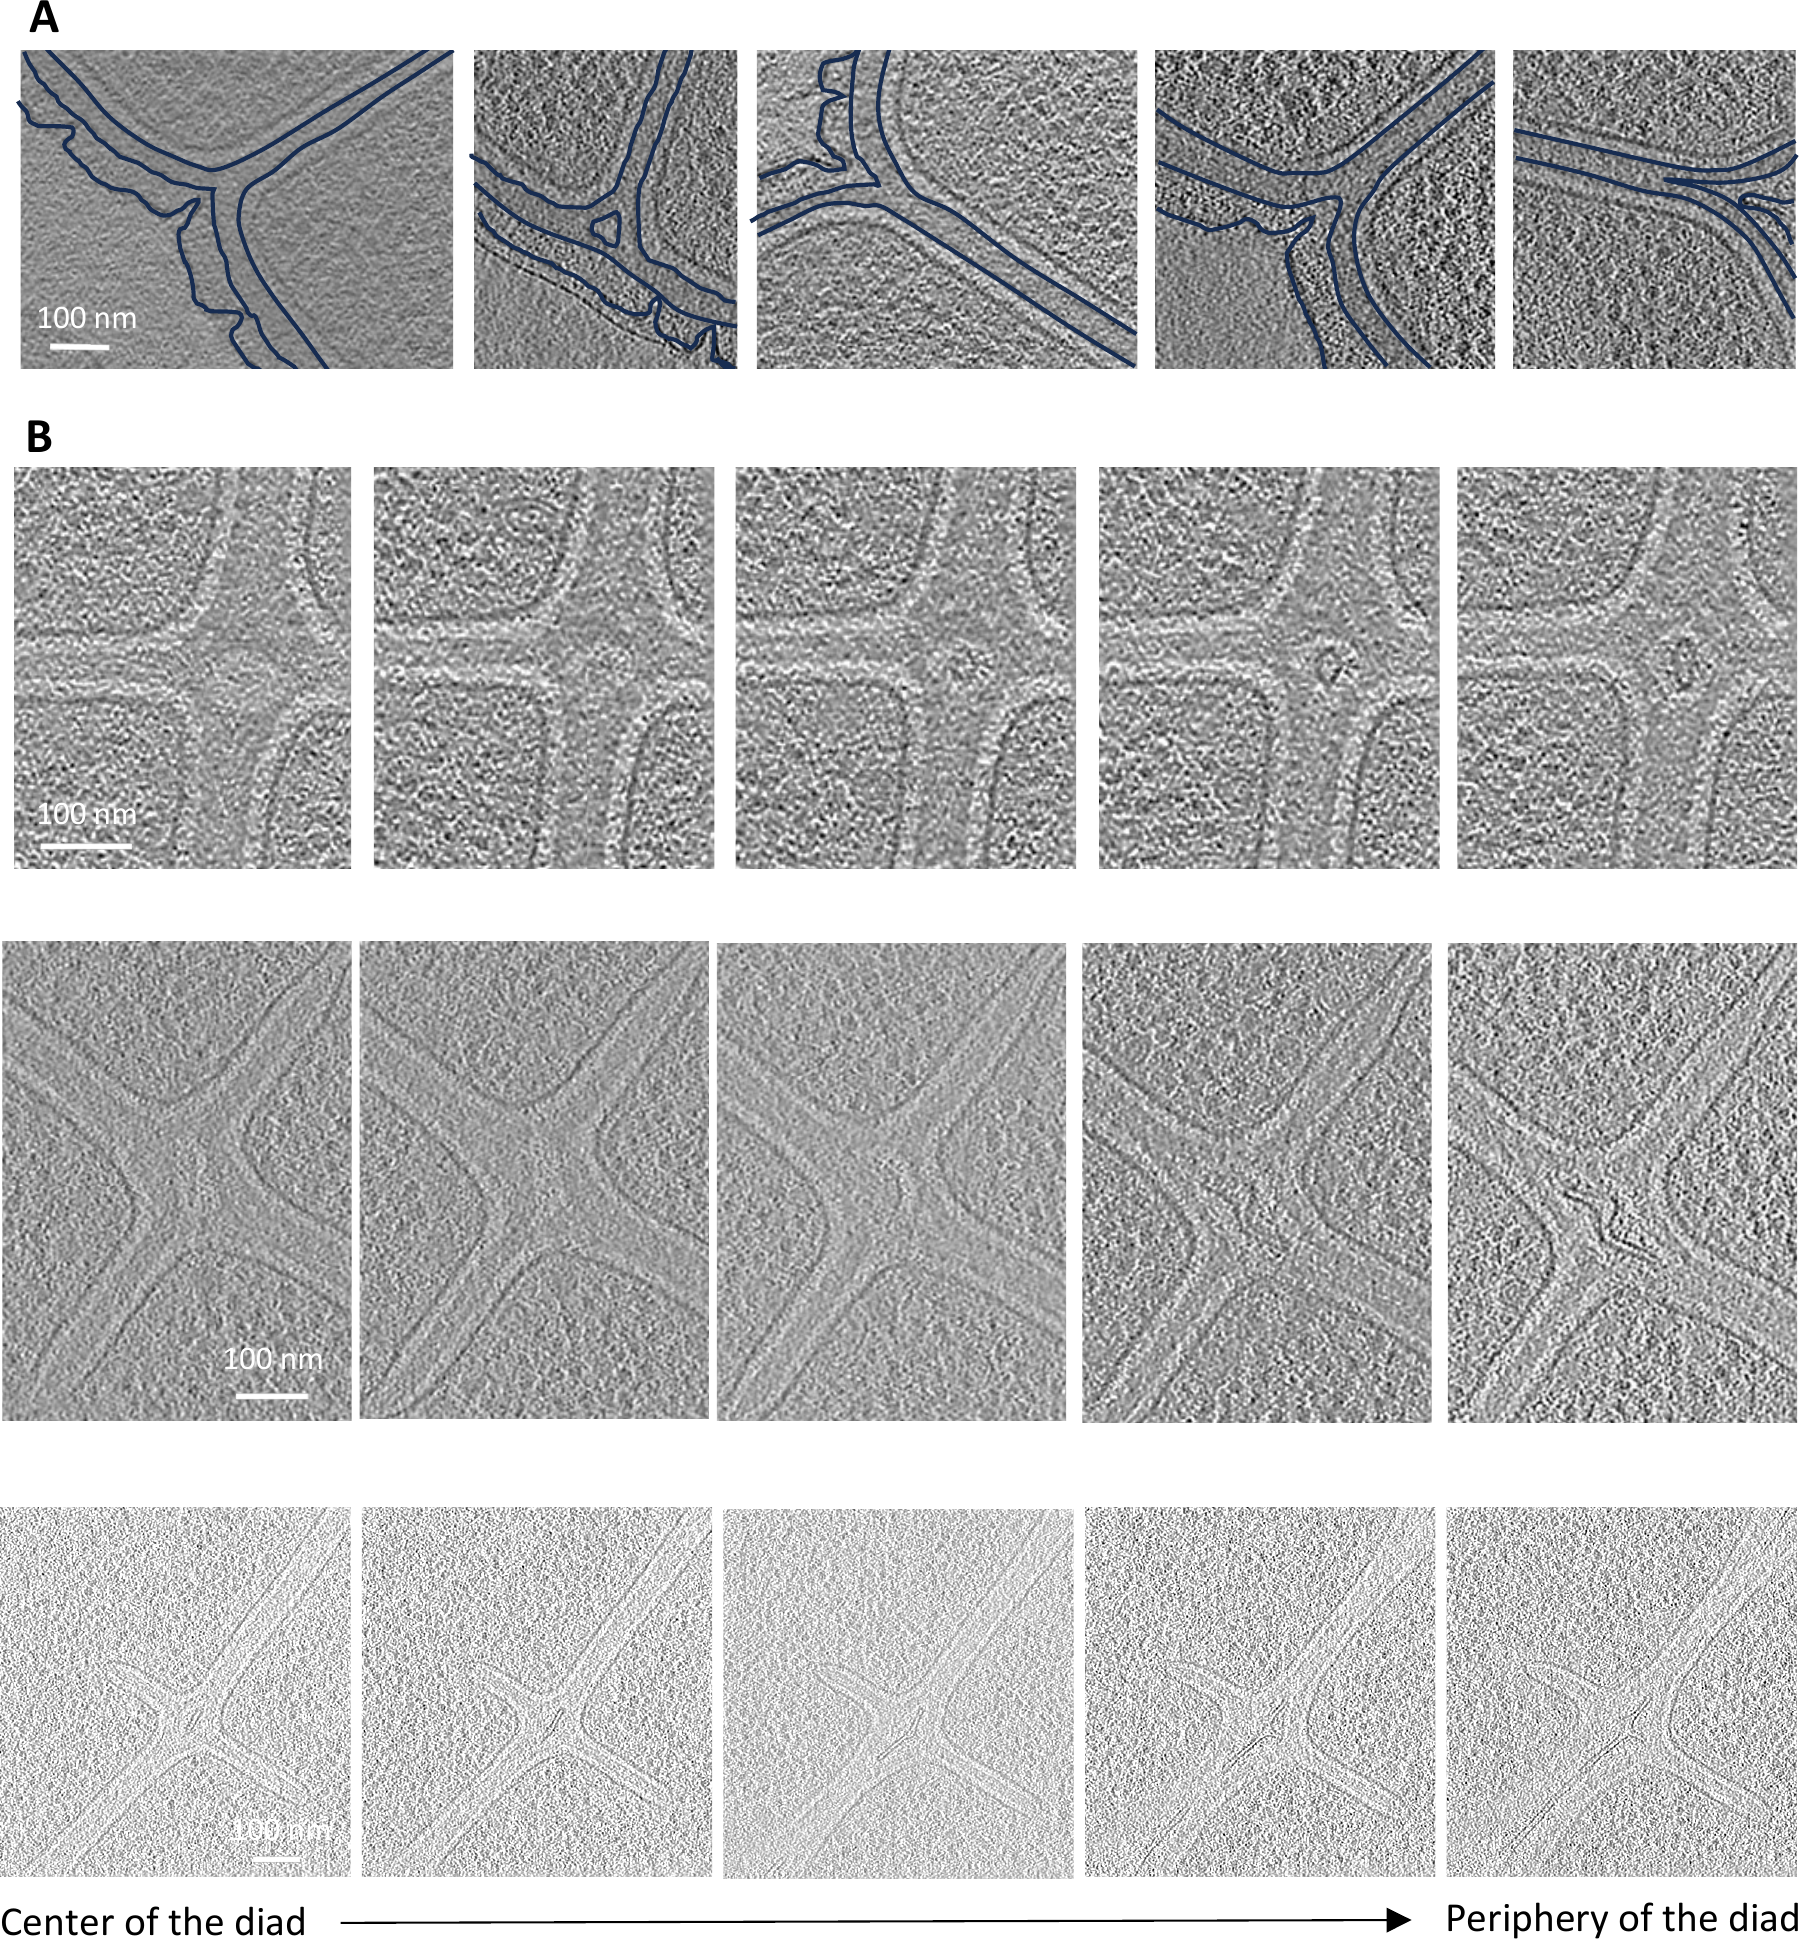
\includegraphics[width=\textwidth]{drad_paper/sfig1.png}
    \caption{TODO}
    \label{drad_sfig1}
\end{figure}

\begin{figure}[ht]
    \centering
    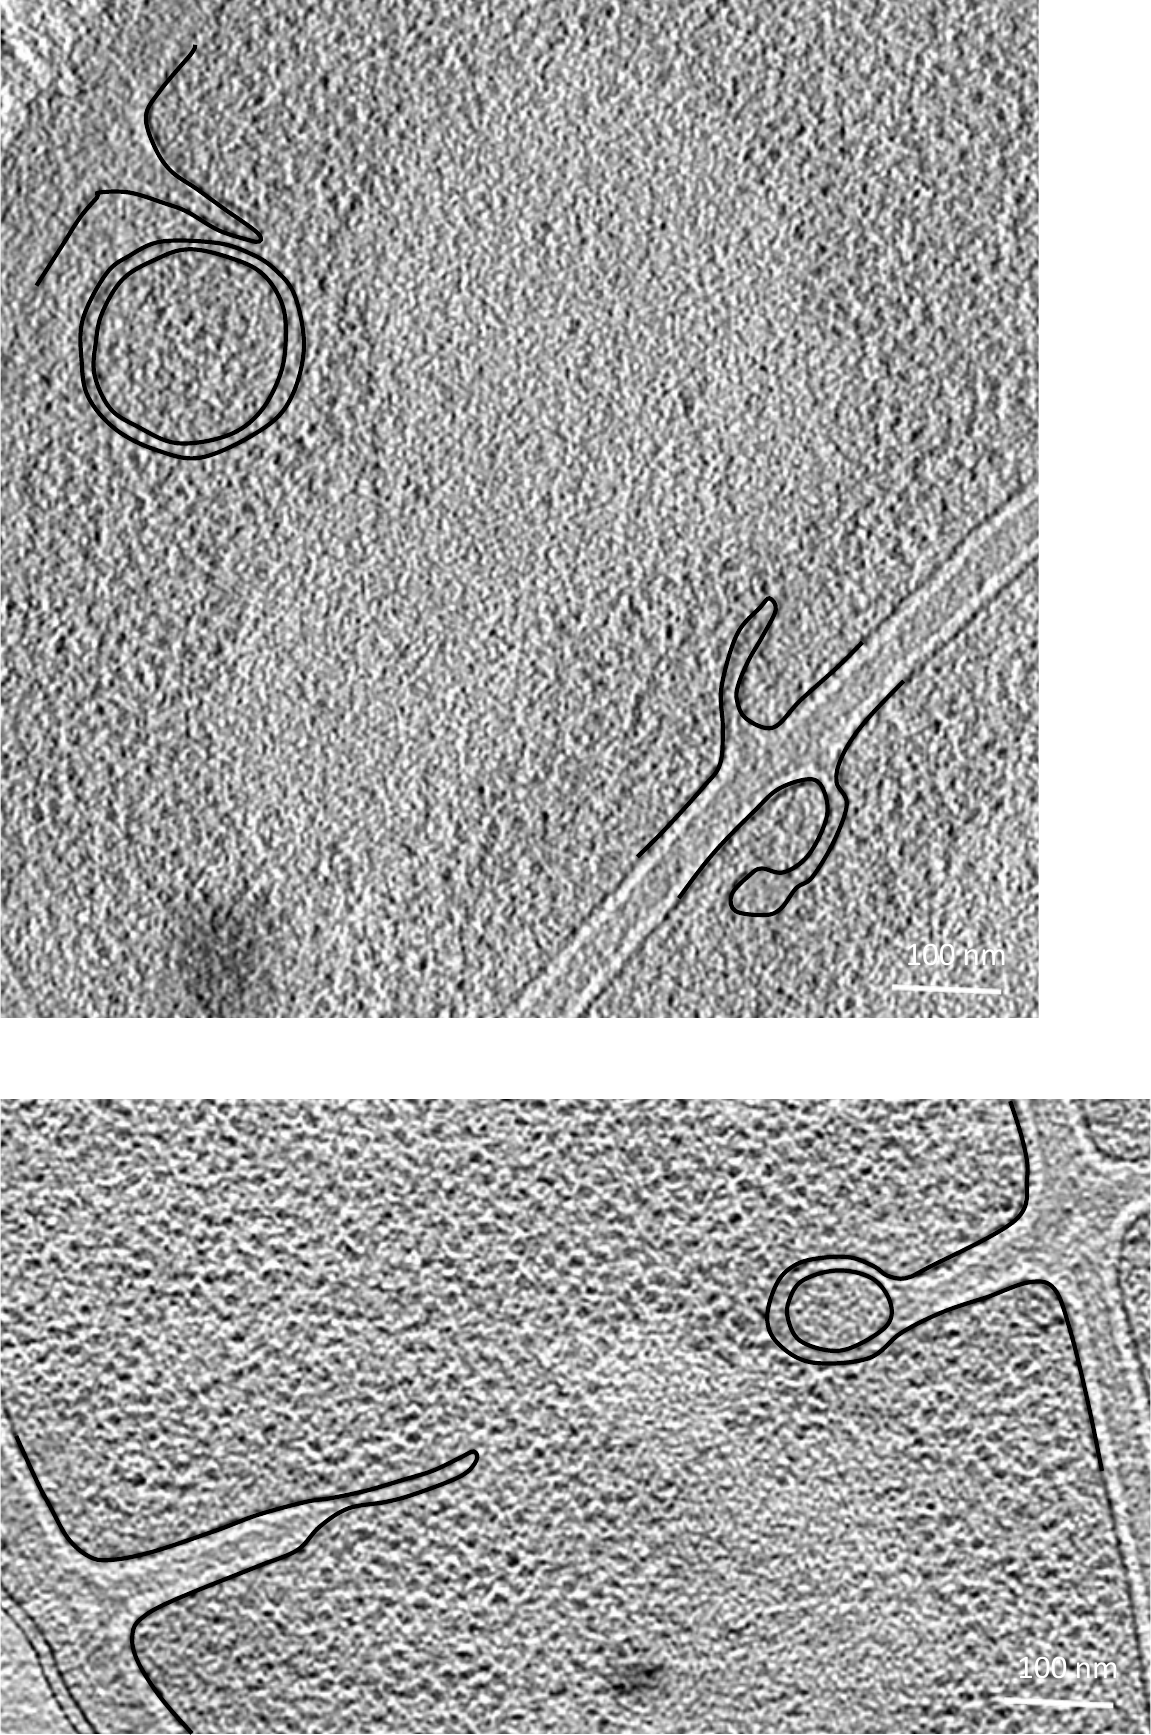
\includegraphics[width=.8\textwidth]{drad_paper/sfig2.png}
    \caption{TODO}
    \label{drad_sfig2}
\end{figure}

\begin{figure}[ht]
    \centering
    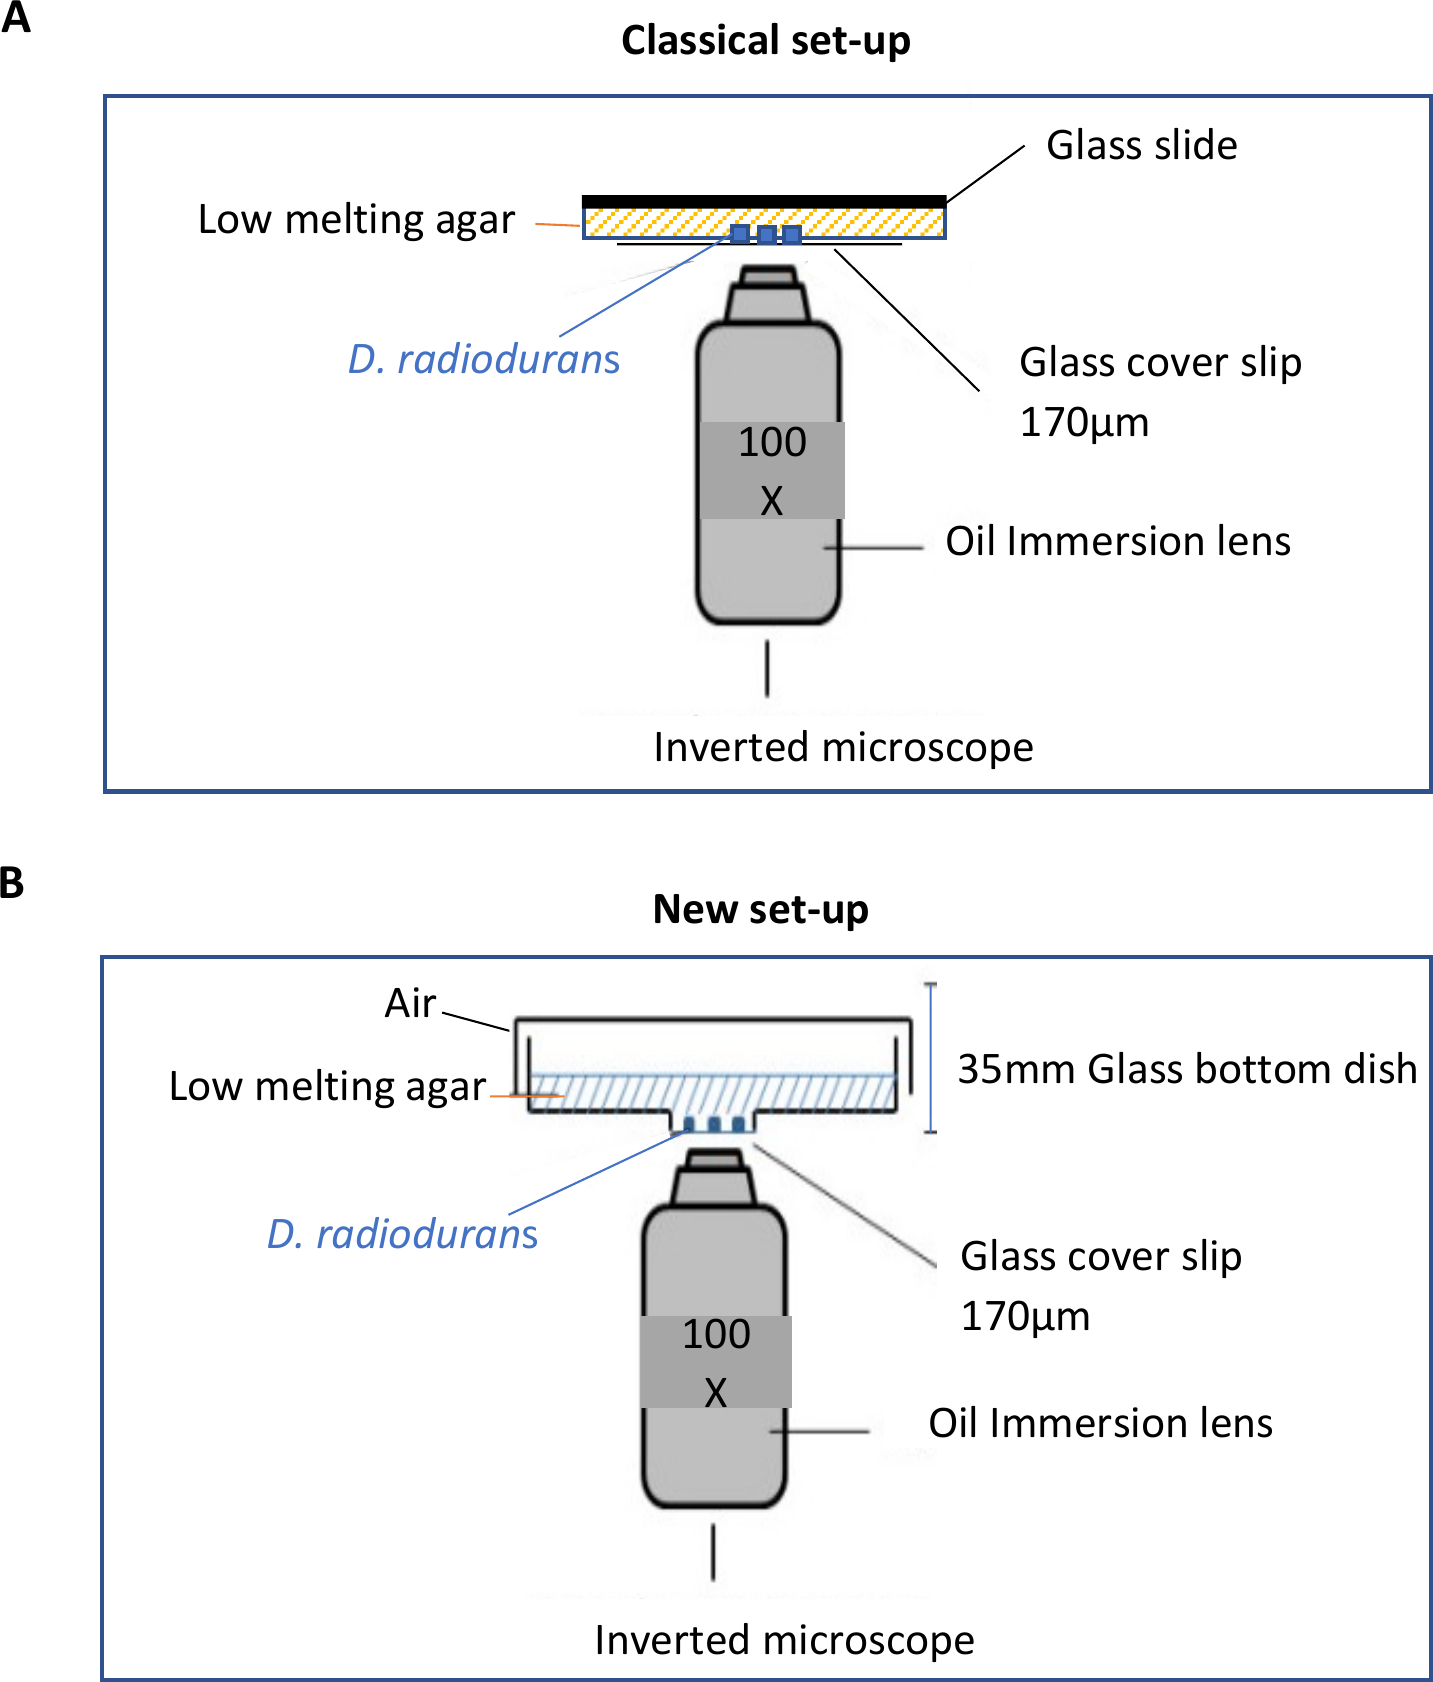
\includegraphics[width=\textwidth]{drad_paper/sfig3.png}
    \caption{TODO}
    \label{drad_sfig3}
\end{figure}

\begin{figure}[ht]
    \centering
    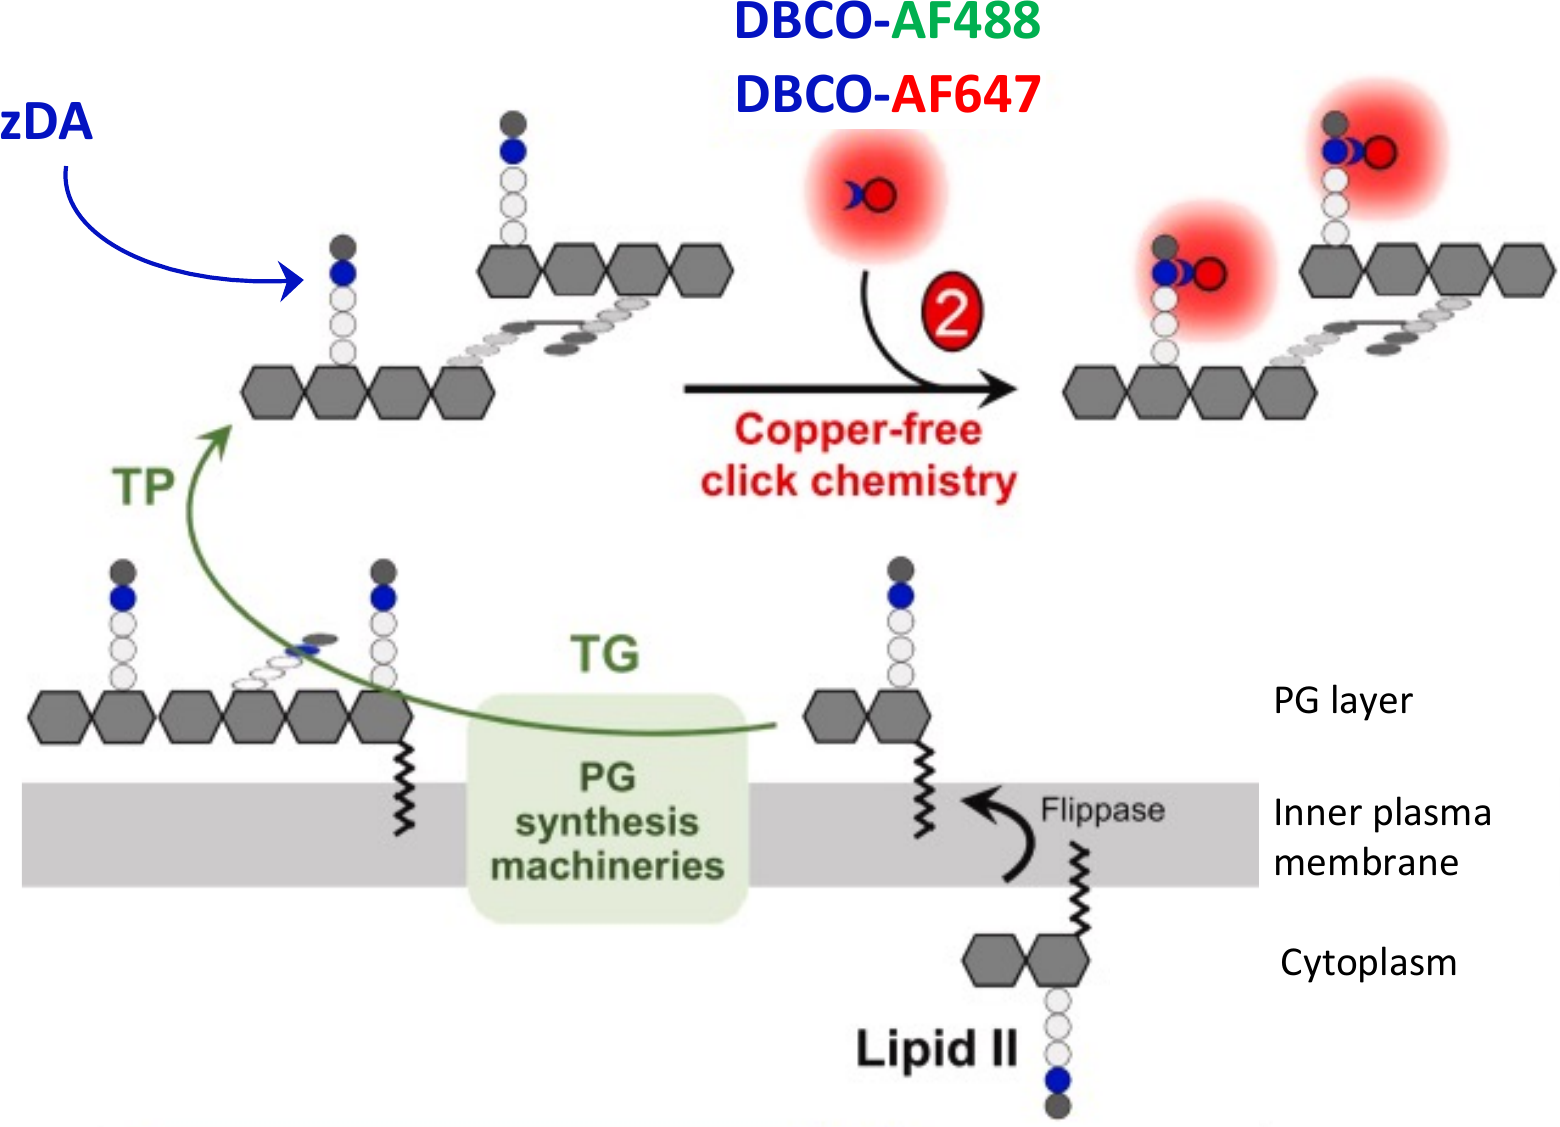
\includegraphics[width=\textwidth]{drad_paper/sfig4.png}
    \caption{TODO}
    \label{drad_sfig4}
\end{figure}

\begin{figure}[ht]
    \centering
    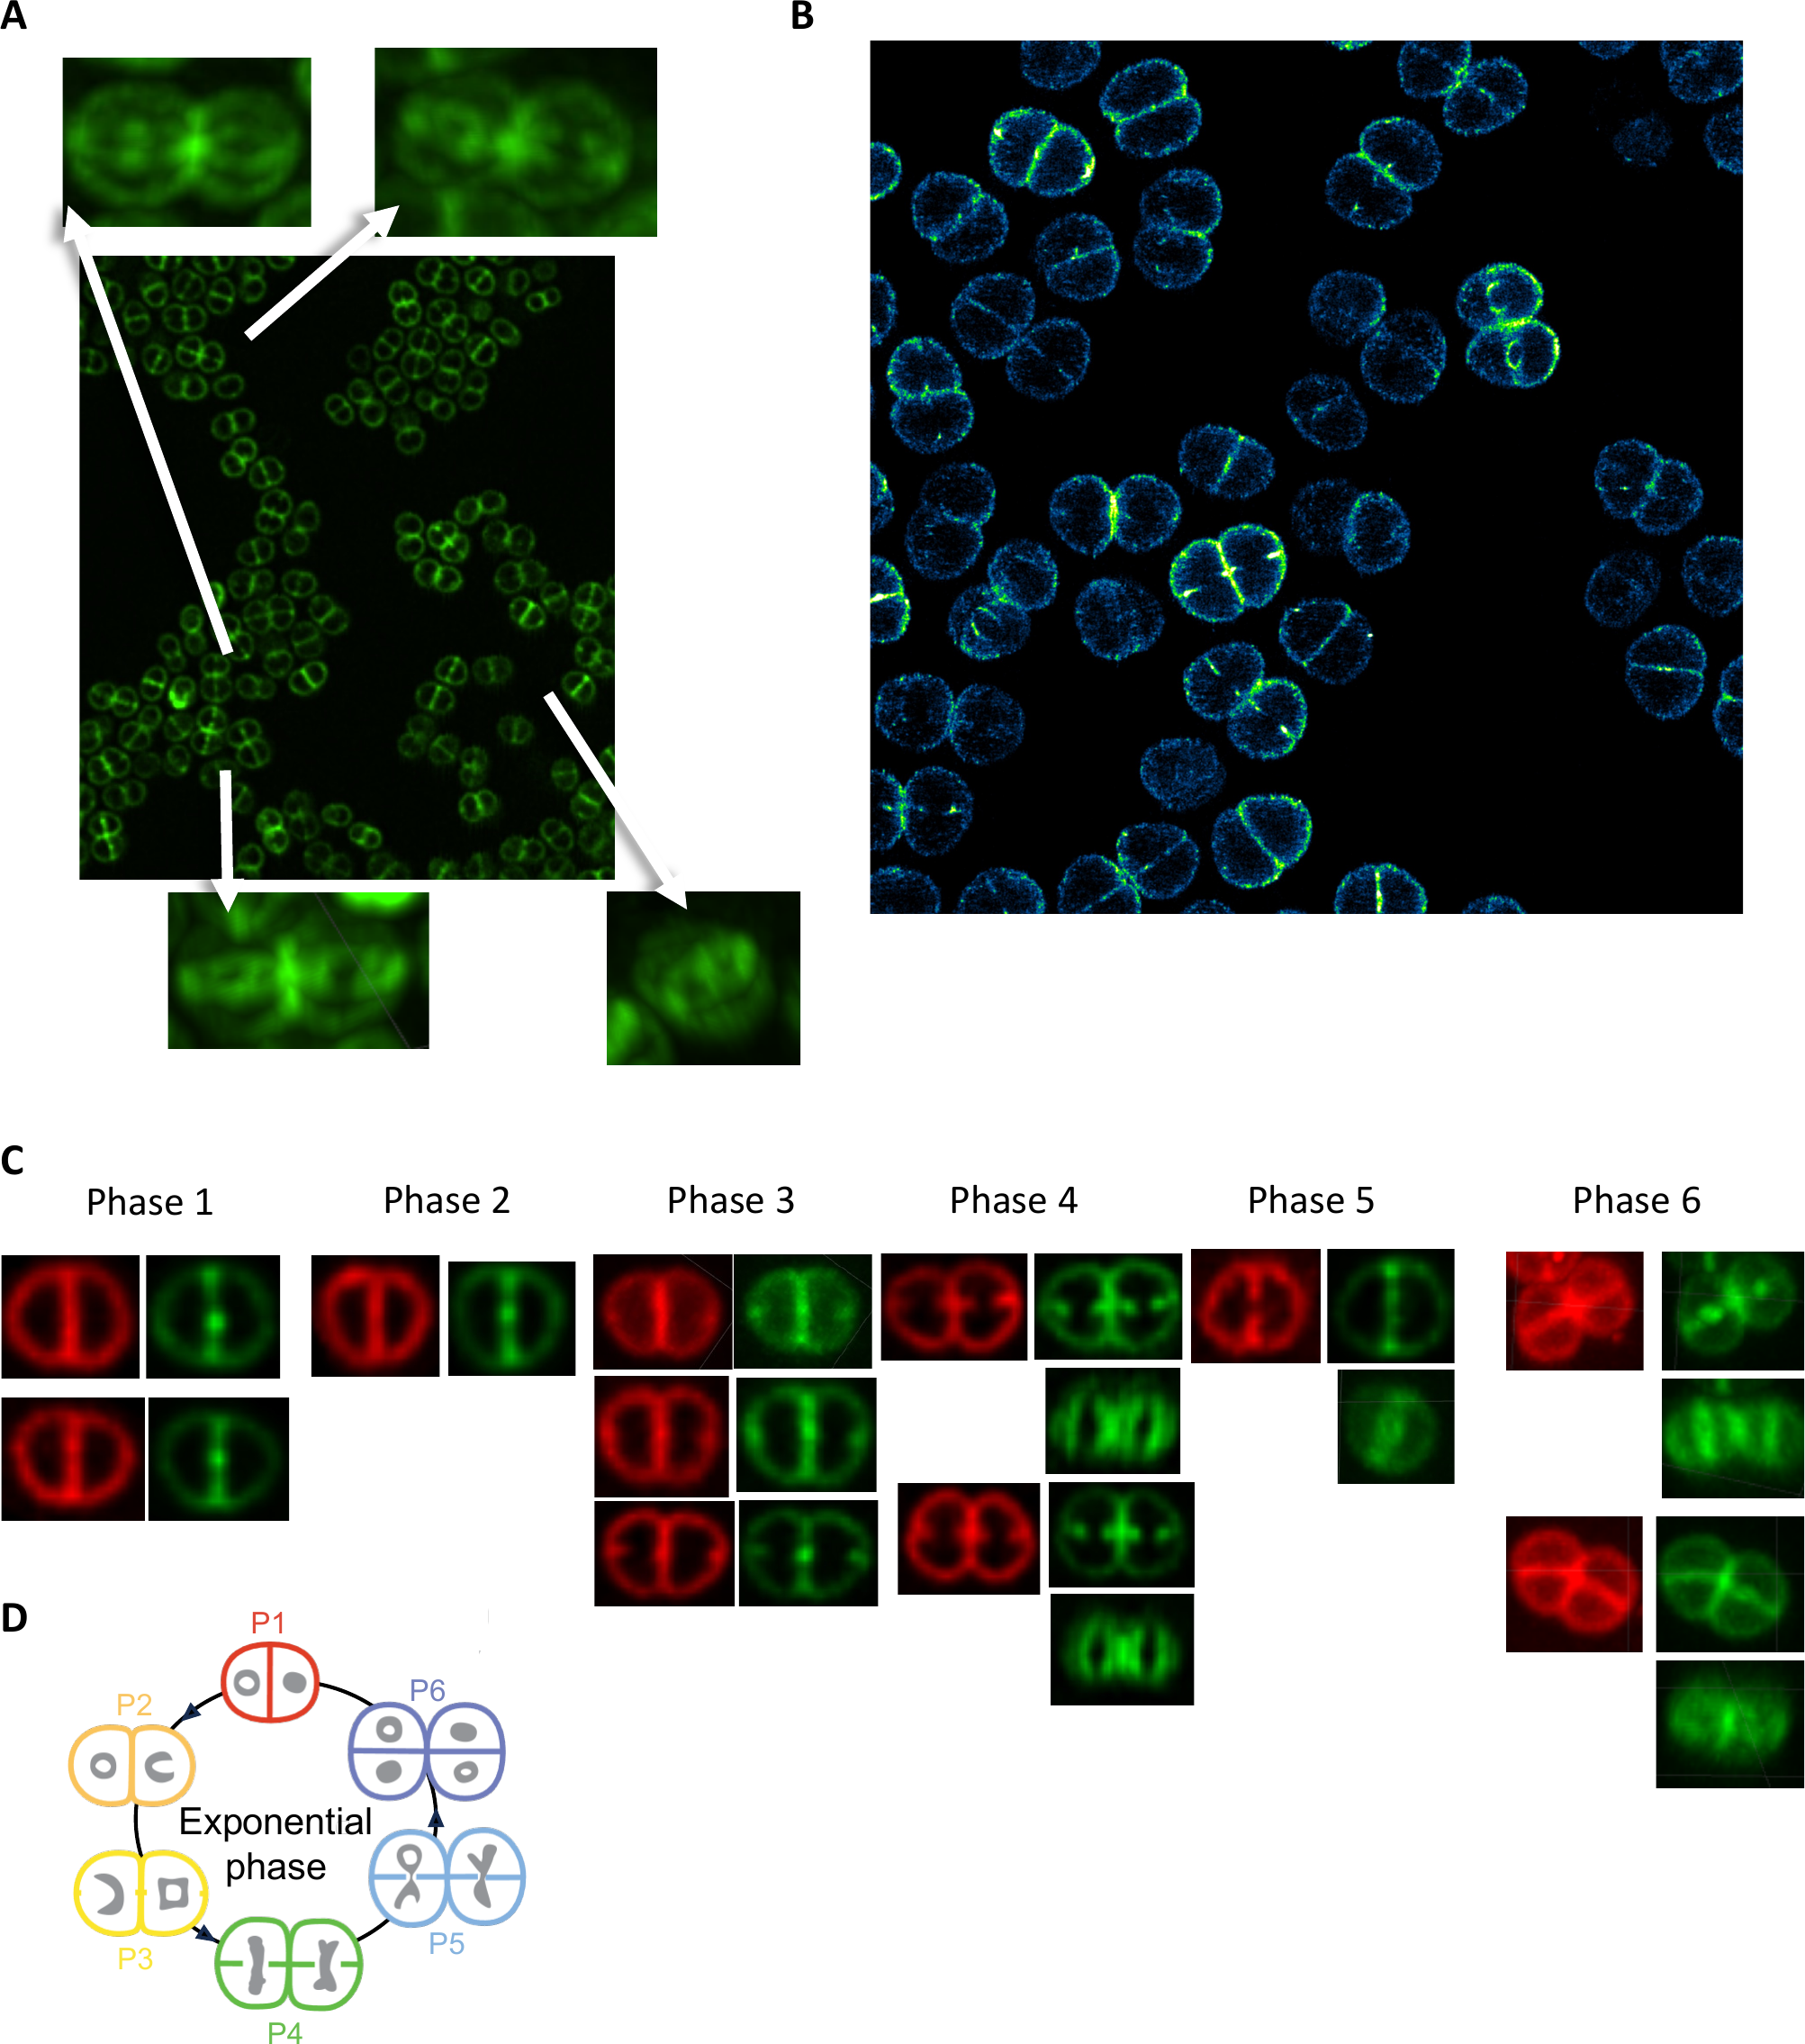
\includegraphics[width=\textwidth]{drad_paper/sfig5.png}
    \caption{TODO}
    \label{drad_sfig5}
\end{figure}

\begin{figure}[ht]
    \centering
    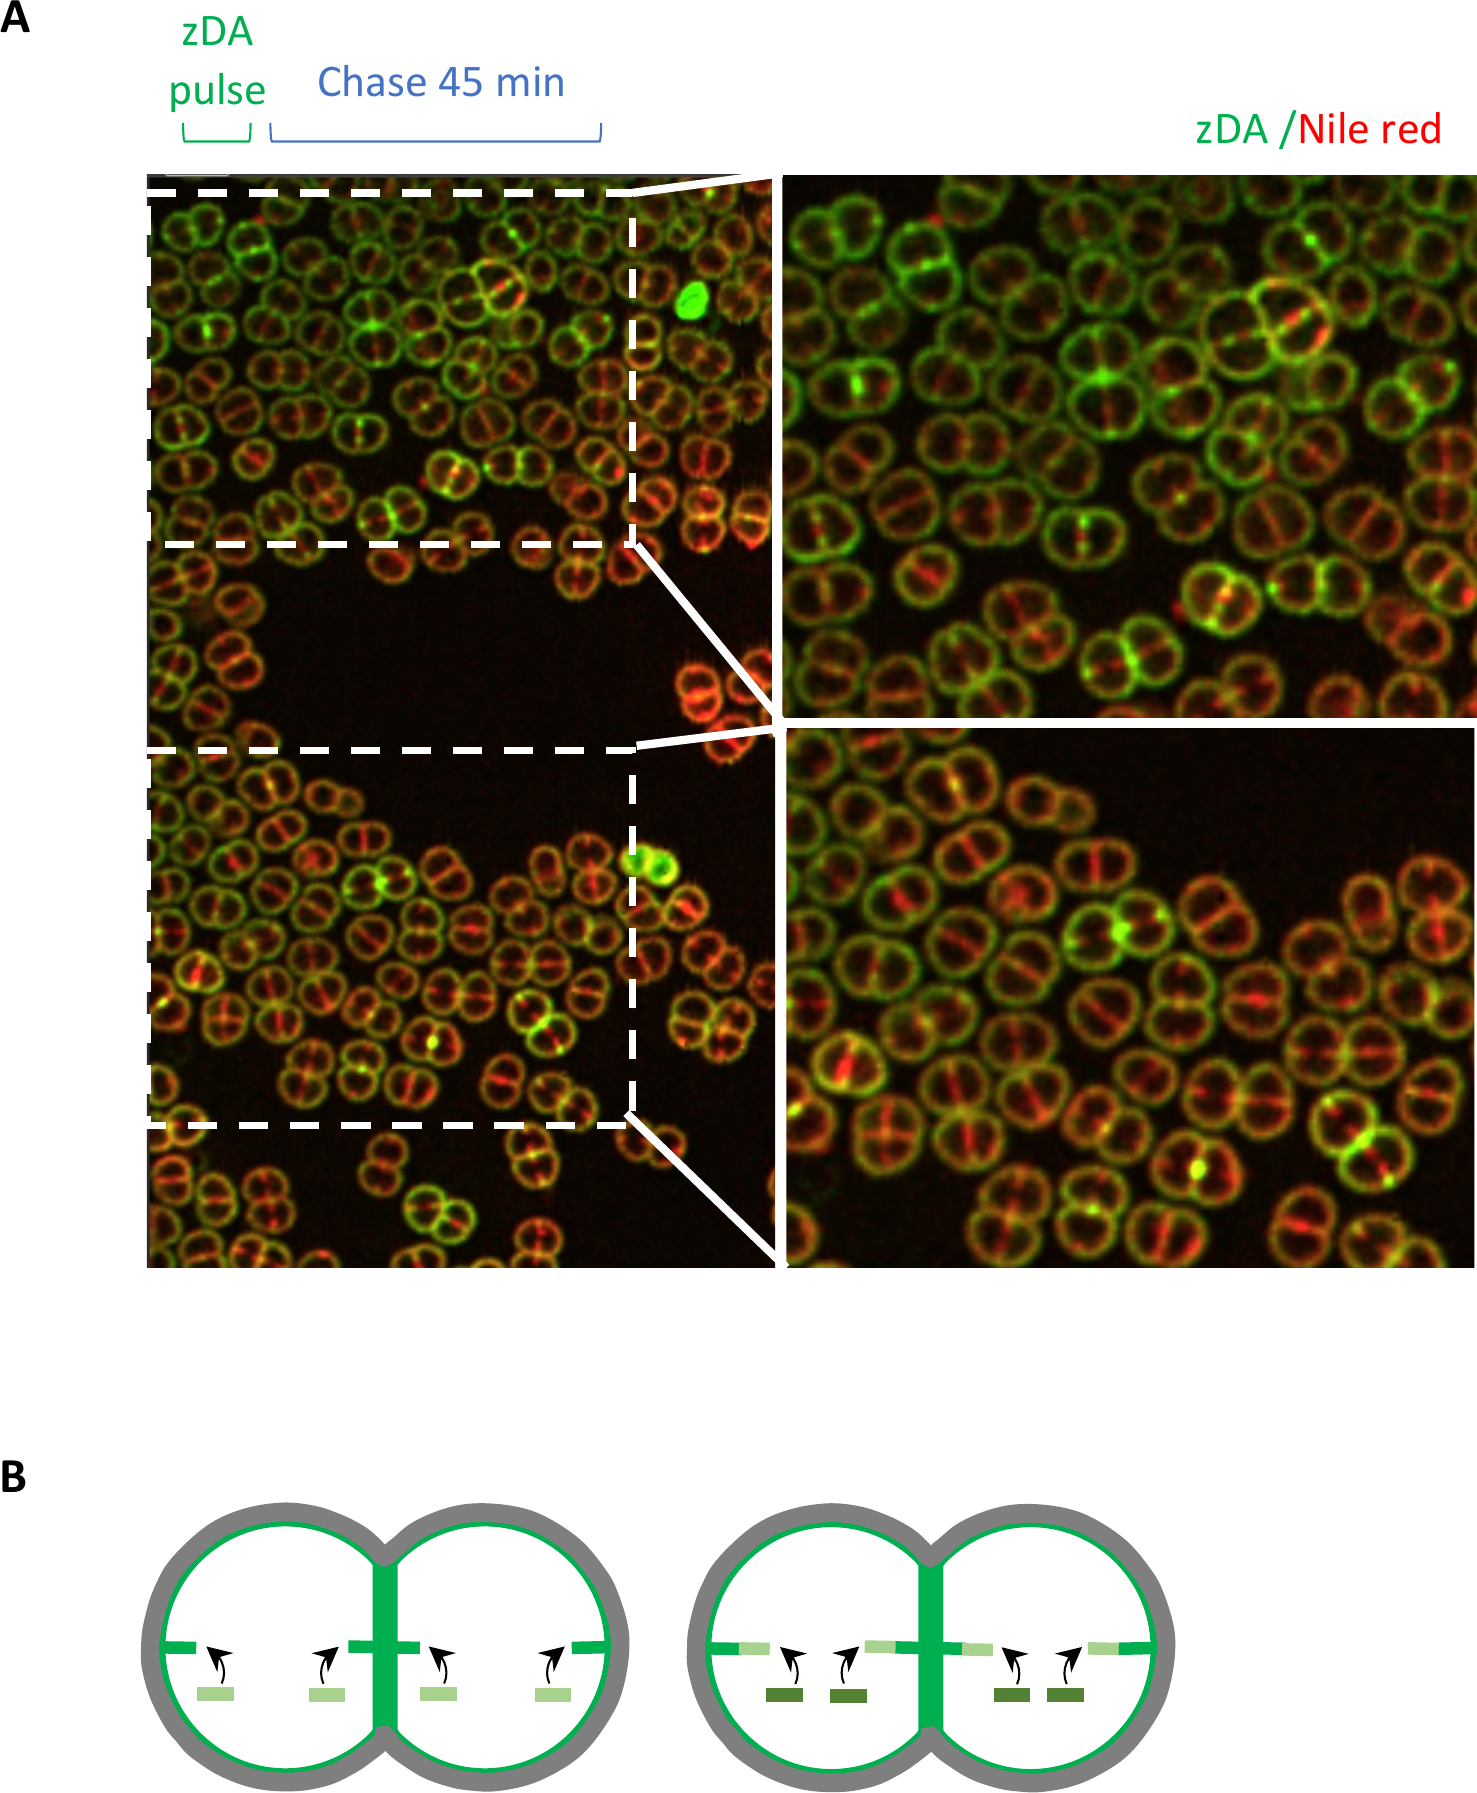
\includegraphics[width=\textwidth]{drad_paper/sfig6.png}
    \caption{TODO}
    \label{drad_sfig6}
\end{figure}

\begin{figure}[ht]
    \centering
    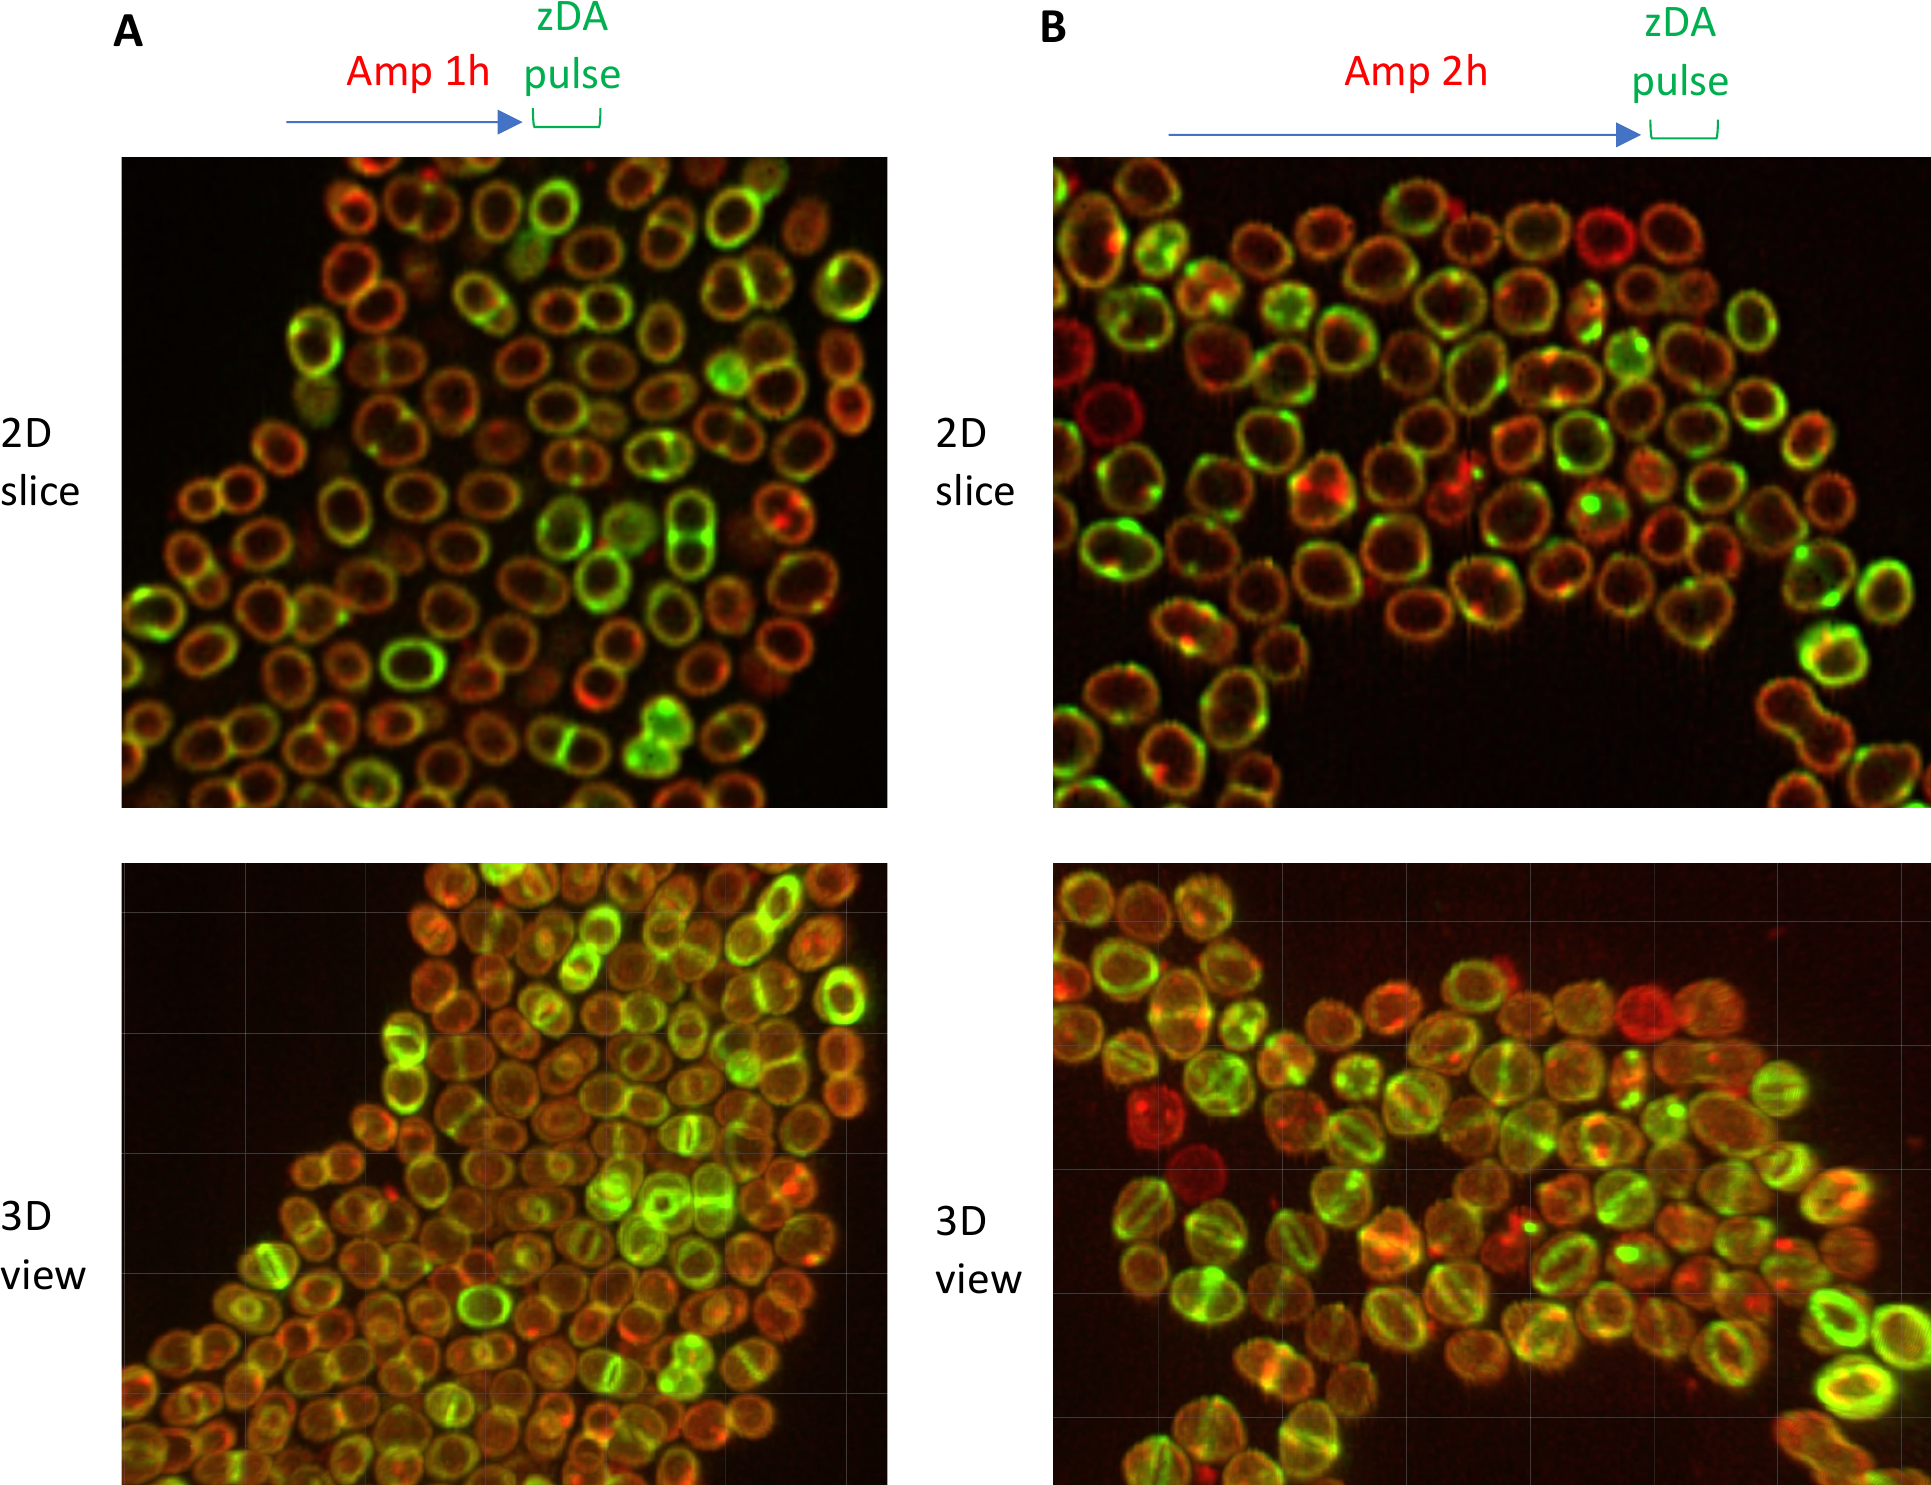
\includegraphics[width=\textwidth]{drad_paper/sfig7.png}
    \caption{TODO}
    \label{drad_sfig7}
\end{figure}

\FloatBarrier
